\documentclass[12pt,letterpaper]{article}
\usepackage[T1]{fontenc}
\usepackage[utf8]{inputenc}
\usepackage{helvet}
\renewcommand{\familydefault}{\sfdefault}
\usepackage[letterpaper,left=0.75in,right=0.75in,top=0.85in,bottom=0.85in,headheight=18pt,headsep=14pt,footskip=26pt]{geometry}
\usepackage{tikz}
\usepackage{pifont}
\usepackage{fancyhdr}
\definecolor{cred}{RGB}{214,39,40}
\definecolor{cblue}{RGB}{31,92,204}
\pagestyle{fancy}
\fancyhf{}
\renewcommand{\headrulewidth}{0pt}
\lhead{Week NN / Patterns you cannot avoid / Grades 4--5}
\lfoot{Bellingham Math Circle / Week NN / NN-45-v1}
\rfoot{\thepage}
\setlength{\parindent}{0pt}
\setlength{\parskip}{4pt}
\linespread{1.12}
\begin{document}
Color each square of a strip red or blue. The strip is good if no three equally spaced squares, such as 2, 5, 8 or 4, 5, 6, are all the same color.
\begin{center}
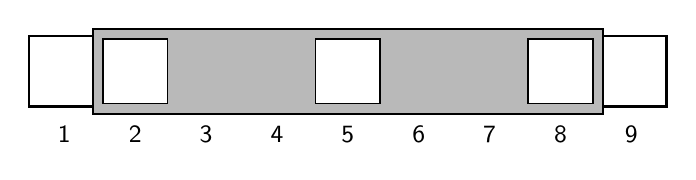
\begin{tikzpicture}
\draw[line width=0.9pt] (0.000,0.000) rectangle (0.900,0.900);
\node[font=\small, anchor=base] at (0.450,-0.450) {1};
\draw[line width=0.9pt] (0.900,0.000) rectangle (1.800,0.900);
\node[font=\small, anchor=base] at (1.350,-0.450) {2};
\draw[line width=0.9pt] (1.800,0.000) rectangle (2.700,0.900);
\node[font=\small, anchor=base] at (2.250,-0.450) {3};
\draw[line width=0.9pt] (2.700,0.000) rectangle (3.600,0.900);
\node[font=\small, anchor=base] at (3.150,-0.450) {4};
\draw[line width=0.9pt] (3.600,0.000) rectangle (4.500,0.900);
\node[font=\small, anchor=base] at (4.050,-0.450) {5};
\draw[line width=0.9pt] (4.500,0.000) rectangle (5.400,0.900);
\node[font=\small, anchor=base] at (4.950,-0.450) {6};
\draw[line width=0.9pt] (5.400,0.000) rectangle (6.300,0.900);
\node[font=\small, anchor=base] at (5.850,-0.450) {7};
\draw[line width=0.9pt] (6.300,0.000) rectangle (7.200,0.900);
\node[font=\small, anchor=base] at (6.750,-0.450) {8};
\draw[line width=0.9pt] (7.200,0.000) rectangle (8.100,0.900);
\node[font=\small, anchor=base] at (7.650,-0.450) {9};
\fill[gray!55, even odd rule] (0.810,-0.090) rectangle (7.290,0.990) (0.940,0.040) rectangle (1.760,0.860) (3.640,0.040) rectangle (4.460,0.860) (6.340,0.040) rectangle (7.160,0.860);
\draw[line width=0.8pt] (0.810,-0.090) rectangle (7.290,0.990);
\draw[line width=0.6pt] (0.940,0.040) rectangle (1.760,0.860);
\draw[line width=0.6pt] (3.640,0.040) rectangle (4.460,0.860);
\draw[line width=0.6pt] (6.340,0.040) rectangle (7.160,0.860);
\end{tikzpicture}
\end{center}\vspace{8pt}
\par\noindent\textbf{Problem 1:} What is the longest strip you can make good? Color your good strips.\par

\vspace{6pt}\begin{center}
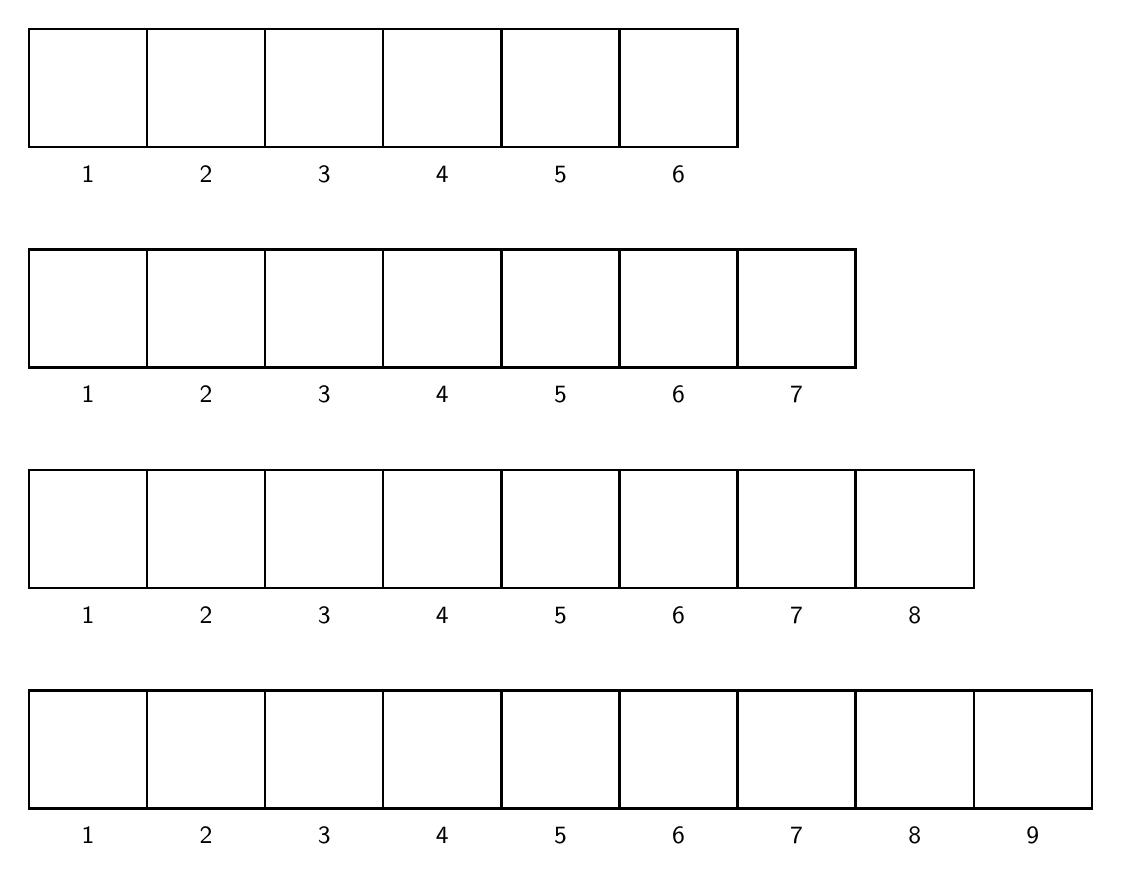
\begin{tikzpicture}
\draw[line width=0.9pt] (0.000,0.000) rectangle (1.500,1.500);
\node[font=\small, anchor=base] at (0.750,-0.450) {1};
\draw[line width=0.9pt] (1.500,0.000) rectangle (3.000,1.500);
\node[font=\small, anchor=base] at (2.250,-0.450) {2};
\draw[line width=0.9pt] (3.000,0.000) rectangle (4.500,1.500);
\node[font=\small, anchor=base] at (3.750,-0.450) {3};
\draw[line width=0.9pt] (4.500,0.000) rectangle (6.000,1.500);
\node[font=\small, anchor=base] at (5.250,-0.450) {4};
\draw[line width=0.9pt] (6.000,0.000) rectangle (7.500,1.500);
\node[font=\small, anchor=base] at (6.750,-0.450) {5};
\draw[line width=0.9pt] (7.500,0.000) rectangle (9.000,1.500);
\node[font=\small, anchor=base] at (8.250,-0.450) {6};
\draw[line width=0.9pt] (0.000,-2.800) rectangle (1.500,-1.300);
\node[font=\small, anchor=base] at (0.750,-3.250) {1};
\draw[line width=0.9pt] (1.500,-2.800) rectangle (3.000,-1.300);
\node[font=\small, anchor=base] at (2.250,-3.250) {2};
\draw[line width=0.9pt] (3.000,-2.800) rectangle (4.500,-1.300);
\node[font=\small, anchor=base] at (3.750,-3.250) {3};
\draw[line width=0.9pt] (4.500,-2.800) rectangle (6.000,-1.300);
\node[font=\small, anchor=base] at (5.250,-3.250) {4};
\draw[line width=0.9pt] (6.000,-2.800) rectangle (7.500,-1.300);
\node[font=\small, anchor=base] at (6.750,-3.250) {5};
\draw[line width=0.9pt] (7.500,-2.800) rectangle (9.000,-1.300);
\node[font=\small, anchor=base] at (8.250,-3.250) {6};
\draw[line width=0.9pt] (9.000,-2.800) rectangle (10.500,-1.300);
\node[font=\small, anchor=base] at (9.750,-3.250) {7};
\draw[line width=0.9pt] (0.000,-5.600) rectangle (1.500,-4.100);
\node[font=\small, anchor=base] at (0.750,-6.050) {1};
\draw[line width=0.9pt] (1.500,-5.600) rectangle (3.000,-4.100);
\node[font=\small, anchor=base] at (2.250,-6.050) {2};
\draw[line width=0.9pt] (3.000,-5.600) rectangle (4.500,-4.100);
\node[font=\small, anchor=base] at (3.750,-6.050) {3};
\draw[line width=0.9pt] (4.500,-5.600) rectangle (6.000,-4.100);
\node[font=\small, anchor=base] at (5.250,-6.050) {4};
\draw[line width=0.9pt] (6.000,-5.600) rectangle (7.500,-4.100);
\node[font=\small, anchor=base] at (6.750,-6.050) {5};
\draw[line width=0.9pt] (7.500,-5.600) rectangle (9.000,-4.100);
\node[font=\small, anchor=base] at (8.250,-6.050) {6};
\draw[line width=0.9pt] (9.000,-5.600) rectangle (10.500,-4.100);
\node[font=\small, anchor=base] at (9.750,-6.050) {7};
\draw[line width=0.9pt] (10.500,-5.600) rectangle (12.000,-4.100);
\node[font=\small, anchor=base] at (11.250,-6.050) {8};
\draw[line width=0.9pt] (0.000,-8.400) rectangle (1.500,-6.900);
\node[font=\small, anchor=base] at (0.750,-8.850) {1};
\draw[line width=0.9pt] (1.500,-8.400) rectangle (3.000,-6.900);
\node[font=\small, anchor=base] at (2.250,-8.850) {2};
\draw[line width=0.9pt] (3.000,-8.400) rectangle (4.500,-6.900);
\node[font=\small, anchor=base] at (3.750,-8.850) {3};
\draw[line width=0.9pt] (4.500,-8.400) rectangle (6.000,-6.900);
\node[font=\small, anchor=base] at (5.250,-8.850) {4};
\draw[line width=0.9pt] (6.000,-8.400) rectangle (7.500,-6.900);
\node[font=\small, anchor=base] at (6.750,-8.850) {5};
\draw[line width=0.9pt] (7.500,-8.400) rectangle (9.000,-6.900);
\node[font=\small, anchor=base] at (8.250,-8.850) {6};
\draw[line width=0.9pt] (9.000,-8.400) rectangle (10.500,-6.900);
\node[font=\small, anchor=base] at (9.750,-8.850) {7};
\draw[line width=0.9pt] (10.500,-8.400) rectangle (12.000,-6.900);
\node[font=\small, anchor=base] at (11.250,-8.850) {8};
\draw[line width=0.9pt] (12.000,-8.400) rectangle (13.500,-6.900);
\node[font=\small, anchor=base] at (12.750,-8.850) {9};
\end{tikzpicture}
\end{center}
\newpage
\par\noindent\textbf{Problem 2:} Find every good way to color a strip of 8 squares.\par

\vspace{6pt}\begin{center}
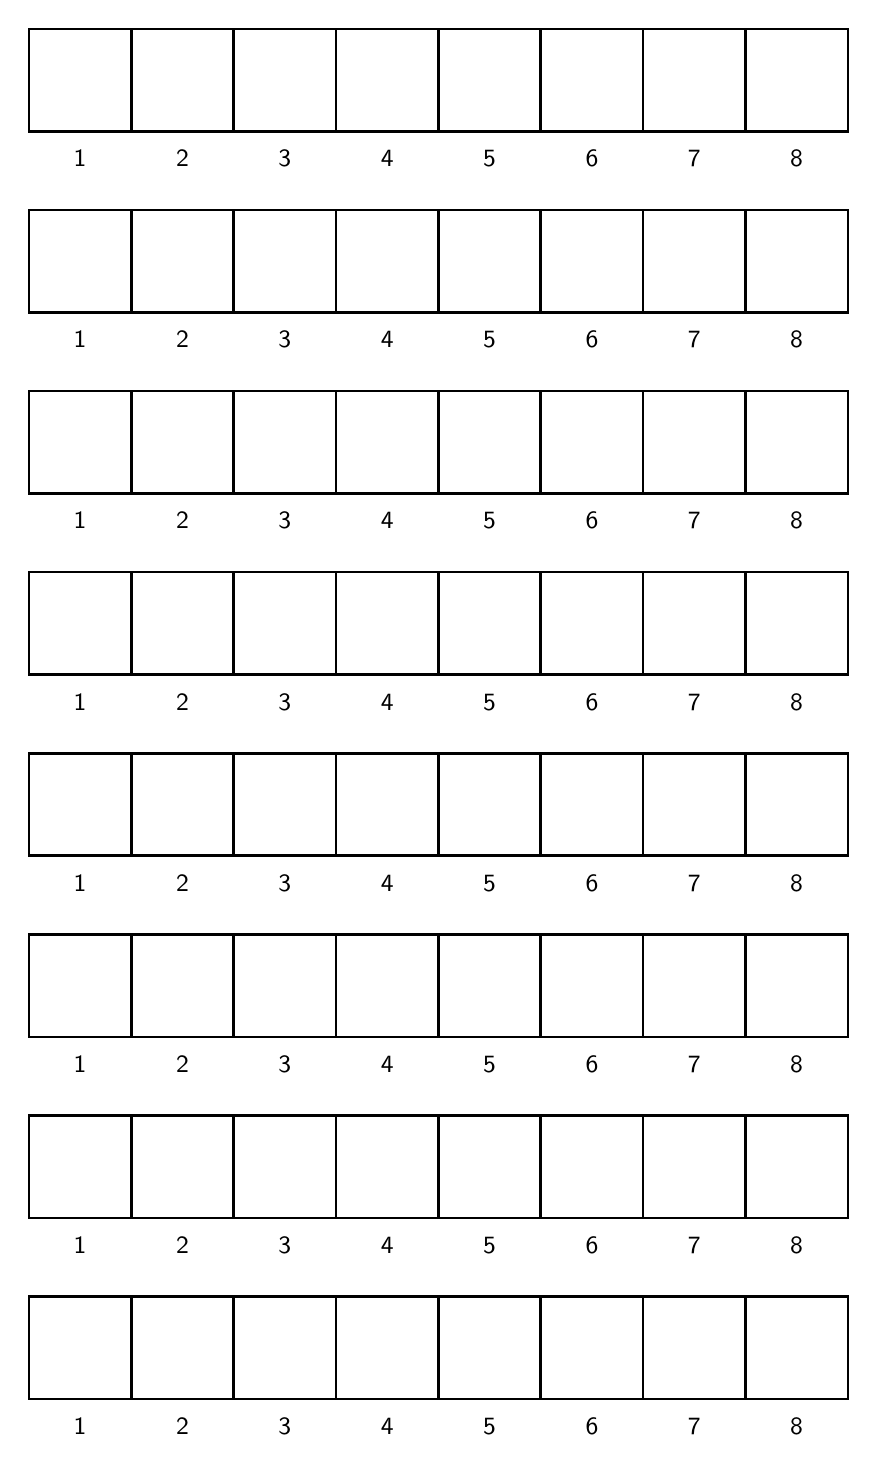
\begin{tikzpicture}
\draw[line width=0.9pt] (0.000,0.000) rectangle (1.300,1.300);
\node[font=\small, anchor=base] at (0.650,-0.450) {1};
\draw[line width=0.9pt] (1.300,0.000) rectangle (2.600,1.300);
\node[font=\small, anchor=base] at (1.950,-0.450) {2};
\draw[line width=0.9pt] (2.600,0.000) rectangle (3.900,1.300);
\node[font=\small, anchor=base] at (3.250,-0.450) {3};
\draw[line width=0.9pt] (3.900,0.000) rectangle (5.200,1.300);
\node[font=\small, anchor=base] at (4.550,-0.450) {4};
\draw[line width=0.9pt] (5.200,0.000) rectangle (6.500,1.300);
\node[font=\small, anchor=base] at (5.850,-0.450) {5};
\draw[line width=0.9pt] (6.500,0.000) rectangle (7.800,1.300);
\node[font=\small, anchor=base] at (7.150,-0.450) {6};
\draw[line width=0.9pt] (7.800,0.000) rectangle (9.100,1.300);
\node[font=\small, anchor=base] at (8.450,-0.450) {7};
\draw[line width=0.9pt] (9.100,0.000) rectangle (10.400,1.300);
\node[font=\small, anchor=base] at (9.750,-0.450) {8};
\draw[line width=0.9pt] (0.000,-2.300) rectangle (1.300,-1.000);
\node[font=\small, anchor=base] at (0.650,-2.750) {1};
\draw[line width=0.9pt] (1.300,-2.300) rectangle (2.600,-1.000);
\node[font=\small, anchor=base] at (1.950,-2.750) {2};
\draw[line width=0.9pt] (2.600,-2.300) rectangle (3.900,-1.000);
\node[font=\small, anchor=base] at (3.250,-2.750) {3};
\draw[line width=0.9pt] (3.900,-2.300) rectangle (5.200,-1.000);
\node[font=\small, anchor=base] at (4.550,-2.750) {4};
\draw[line width=0.9pt] (5.200,-2.300) rectangle (6.500,-1.000);
\node[font=\small, anchor=base] at (5.850,-2.750) {5};
\draw[line width=0.9pt] (6.500,-2.300) rectangle (7.800,-1.000);
\node[font=\small, anchor=base] at (7.150,-2.750) {6};
\draw[line width=0.9pt] (7.800,-2.300) rectangle (9.100,-1.000);
\node[font=\small, anchor=base] at (8.450,-2.750) {7};
\draw[line width=0.9pt] (9.100,-2.300) rectangle (10.400,-1.000);
\node[font=\small, anchor=base] at (9.750,-2.750) {8};
\draw[line width=0.9pt] (0.000,-4.600) rectangle (1.300,-3.300);
\node[font=\small, anchor=base] at (0.650,-5.050) {1};
\draw[line width=0.9pt] (1.300,-4.600) rectangle (2.600,-3.300);
\node[font=\small, anchor=base] at (1.950,-5.050) {2};
\draw[line width=0.9pt] (2.600,-4.600) rectangle (3.900,-3.300);
\node[font=\small, anchor=base] at (3.250,-5.050) {3};
\draw[line width=0.9pt] (3.900,-4.600) rectangle (5.200,-3.300);
\node[font=\small, anchor=base] at (4.550,-5.050) {4};
\draw[line width=0.9pt] (5.200,-4.600) rectangle (6.500,-3.300);
\node[font=\small, anchor=base] at (5.850,-5.050) {5};
\draw[line width=0.9pt] (6.500,-4.600) rectangle (7.800,-3.300);
\node[font=\small, anchor=base] at (7.150,-5.050) {6};
\draw[line width=0.9pt] (7.800,-4.600) rectangle (9.100,-3.300);
\node[font=\small, anchor=base] at (8.450,-5.050) {7};
\draw[line width=0.9pt] (9.100,-4.600) rectangle (10.400,-3.300);
\node[font=\small, anchor=base] at (9.750,-5.050) {8};
\draw[line width=0.9pt] (0.000,-6.900) rectangle (1.300,-5.600);
\node[font=\small, anchor=base] at (0.650,-7.350) {1};
\draw[line width=0.9pt] (1.300,-6.900) rectangle (2.600,-5.600);
\node[font=\small, anchor=base] at (1.950,-7.350) {2};
\draw[line width=0.9pt] (2.600,-6.900) rectangle (3.900,-5.600);
\node[font=\small, anchor=base] at (3.250,-7.350) {3};
\draw[line width=0.9pt] (3.900,-6.900) rectangle (5.200,-5.600);
\node[font=\small, anchor=base] at (4.550,-7.350) {4};
\draw[line width=0.9pt] (5.200,-6.900) rectangle (6.500,-5.600);
\node[font=\small, anchor=base] at (5.850,-7.350) {5};
\draw[line width=0.9pt] (6.500,-6.900) rectangle (7.800,-5.600);
\node[font=\small, anchor=base] at (7.150,-7.350) {6};
\draw[line width=0.9pt] (7.800,-6.900) rectangle (9.100,-5.600);
\node[font=\small, anchor=base] at (8.450,-7.350) {7};
\draw[line width=0.9pt] (9.100,-6.900) rectangle (10.400,-5.600);
\node[font=\small, anchor=base] at (9.750,-7.350) {8};
\draw[line width=0.9pt] (0.000,-9.200) rectangle (1.300,-7.900);
\node[font=\small, anchor=base] at (0.650,-9.650) {1};
\draw[line width=0.9pt] (1.300,-9.200) rectangle (2.600,-7.900);
\node[font=\small, anchor=base] at (1.950,-9.650) {2};
\draw[line width=0.9pt] (2.600,-9.200) rectangle (3.900,-7.900);
\node[font=\small, anchor=base] at (3.250,-9.650) {3};
\draw[line width=0.9pt] (3.900,-9.200) rectangle (5.200,-7.900);
\node[font=\small, anchor=base] at (4.550,-9.650) {4};
\draw[line width=0.9pt] (5.200,-9.200) rectangle (6.500,-7.900);
\node[font=\small, anchor=base] at (5.850,-9.650) {5};
\draw[line width=0.9pt] (6.500,-9.200) rectangle (7.800,-7.900);
\node[font=\small, anchor=base] at (7.150,-9.650) {6};
\draw[line width=0.9pt] (7.800,-9.200) rectangle (9.100,-7.900);
\node[font=\small, anchor=base] at (8.450,-9.650) {7};
\draw[line width=0.9pt] (9.100,-9.200) rectangle (10.400,-7.900);
\node[font=\small, anchor=base] at (9.750,-9.650) {8};
\draw[line width=0.9pt] (0.000,-11.500) rectangle (1.300,-10.200);
\node[font=\small, anchor=base] at (0.650,-11.950) {1};
\draw[line width=0.9pt] (1.300,-11.500) rectangle (2.600,-10.200);
\node[font=\small, anchor=base] at (1.950,-11.950) {2};
\draw[line width=0.9pt] (2.600,-11.500) rectangle (3.900,-10.200);
\node[font=\small, anchor=base] at (3.250,-11.950) {3};
\draw[line width=0.9pt] (3.900,-11.500) rectangle (5.200,-10.200);
\node[font=\small, anchor=base] at (4.550,-11.950) {4};
\draw[line width=0.9pt] (5.200,-11.500) rectangle (6.500,-10.200);
\node[font=\small, anchor=base] at (5.850,-11.950) {5};
\draw[line width=0.9pt] (6.500,-11.500) rectangle (7.800,-10.200);
\node[font=\small, anchor=base] at (7.150,-11.950) {6};
\draw[line width=0.9pt] (7.800,-11.500) rectangle (9.100,-10.200);
\node[font=\small, anchor=base] at (8.450,-11.950) {7};
\draw[line width=0.9pt] (9.100,-11.500) rectangle (10.400,-10.200);
\node[font=\small, anchor=base] at (9.750,-11.950) {8};
\draw[line width=0.9pt] (0.000,-13.800) rectangle (1.300,-12.500);
\node[font=\small, anchor=base] at (0.650,-14.250) {1};
\draw[line width=0.9pt] (1.300,-13.800) rectangle (2.600,-12.500);
\node[font=\small, anchor=base] at (1.950,-14.250) {2};
\draw[line width=0.9pt] (2.600,-13.800) rectangle (3.900,-12.500);
\node[font=\small, anchor=base] at (3.250,-14.250) {3};
\draw[line width=0.9pt] (3.900,-13.800) rectangle (5.200,-12.500);
\node[font=\small, anchor=base] at (4.550,-14.250) {4};
\draw[line width=0.9pt] (5.200,-13.800) rectangle (6.500,-12.500);
\node[font=\small, anchor=base] at (5.850,-14.250) {5};
\draw[line width=0.9pt] (6.500,-13.800) rectangle (7.800,-12.500);
\node[font=\small, anchor=base] at (7.150,-14.250) {6};
\draw[line width=0.9pt] (7.800,-13.800) rectangle (9.100,-12.500);
\node[font=\small, anchor=base] at (8.450,-14.250) {7};
\draw[line width=0.9pt] (9.100,-13.800) rectangle (10.400,-12.500);
\node[font=\small, anchor=base] at (9.750,-14.250) {8};
\draw[line width=0.9pt] (0.000,-16.100) rectangle (1.300,-14.800);
\node[font=\small, anchor=base] at (0.650,-16.550) {1};
\draw[line width=0.9pt] (1.300,-16.100) rectangle (2.600,-14.800);
\node[font=\small, anchor=base] at (1.950,-16.550) {2};
\draw[line width=0.9pt] (2.600,-16.100) rectangle (3.900,-14.800);
\node[font=\small, anchor=base] at (3.250,-16.550) {3};
\draw[line width=0.9pt] (3.900,-16.100) rectangle (5.200,-14.800);
\node[font=\small, anchor=base] at (4.550,-16.550) {4};
\draw[line width=0.9pt] (5.200,-16.100) rectangle (6.500,-14.800);
\node[font=\small, anchor=base] at (5.850,-16.550) {5};
\draw[line width=0.9pt] (6.500,-16.100) rectangle (7.800,-14.800);
\node[font=\small, anchor=base] at (7.150,-16.550) {6};
\draw[line width=0.9pt] (7.800,-16.100) rectangle (9.100,-14.800);
\node[font=\small, anchor=base] at (8.450,-16.550) {7};
\draw[line width=0.9pt] (9.100,-16.100) rectangle (10.400,-14.800);
\node[font=\small, anchor=base] at (9.750,-16.550) {8};
\end{tikzpicture}
\end{center}
\newpage
\par\noindent\textbf{Problem 3:} Can a strip of 9 squares be good? Explain how you know.\par

\vspace{6pt}\begin{center}
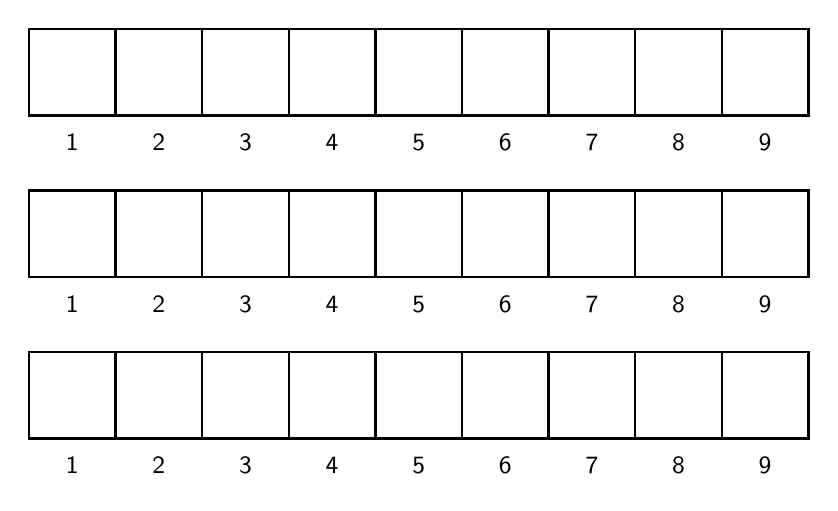
\begin{tikzpicture}
\draw[line width=0.9pt] (0.000,0.000) rectangle (1.100,1.100);
\node[font=\small, anchor=base] at (0.550,-0.450) {1};
\draw[line width=0.9pt] (1.100,0.000) rectangle (2.200,1.100);
\node[font=\small, anchor=base] at (1.650,-0.450) {2};
\draw[line width=0.9pt] (2.200,0.000) rectangle (3.300,1.100);
\node[font=\small, anchor=base] at (2.750,-0.450) {3};
\draw[line width=0.9pt] (3.300,0.000) rectangle (4.400,1.100);
\node[font=\small, anchor=base] at (3.850,-0.450) {4};
\draw[line width=0.9pt] (4.400,0.000) rectangle (5.500,1.100);
\node[font=\small, anchor=base] at (4.950,-0.450) {5};
\draw[line width=0.9pt] (5.500,0.000) rectangle (6.600,1.100);
\node[font=\small, anchor=base] at (6.050,-0.450) {6};
\draw[line width=0.9pt] (6.600,0.000) rectangle (7.700,1.100);
\node[font=\small, anchor=base] at (7.150,-0.450) {7};
\draw[line width=0.9pt] (7.700,0.000) rectangle (8.800,1.100);
\node[font=\small, anchor=base] at (8.250,-0.450) {8};
\draw[line width=0.9pt] (8.800,0.000) rectangle (9.900,1.100);
\node[font=\small, anchor=base] at (9.350,-0.450) {9};
\draw[line width=0.9pt] (0.000,-2.050) rectangle (1.100,-0.950);
\node[font=\small, anchor=base] at (0.550,-2.500) {1};
\draw[line width=0.9pt] (1.100,-2.050) rectangle (2.200,-0.950);
\node[font=\small, anchor=base] at (1.650,-2.500) {2};
\draw[line width=0.9pt] (2.200,-2.050) rectangle (3.300,-0.950);
\node[font=\small, anchor=base] at (2.750,-2.500) {3};
\draw[line width=0.9pt] (3.300,-2.050) rectangle (4.400,-0.950);
\node[font=\small, anchor=base] at (3.850,-2.500) {4};
\draw[line width=0.9pt] (4.400,-2.050) rectangle (5.500,-0.950);
\node[font=\small, anchor=base] at (4.950,-2.500) {5};
\draw[line width=0.9pt] (5.500,-2.050) rectangle (6.600,-0.950);
\node[font=\small, anchor=base] at (6.050,-2.500) {6};
\draw[line width=0.9pt] (6.600,-2.050) rectangle (7.700,-0.950);
\node[font=\small, anchor=base] at (7.150,-2.500) {7};
\draw[line width=0.9pt] (7.700,-2.050) rectangle (8.800,-0.950);
\node[font=\small, anchor=base] at (8.250,-2.500) {8};
\draw[line width=0.9pt] (8.800,-2.050) rectangle (9.900,-0.950);
\node[font=\small, anchor=base] at (9.350,-2.500) {9};
\draw[line width=0.9pt] (0.000,-4.100) rectangle (1.100,-3.000);
\node[font=\small, anchor=base] at (0.550,-4.550) {1};
\draw[line width=0.9pt] (1.100,-4.100) rectangle (2.200,-3.000);
\node[font=\small, anchor=base] at (1.650,-4.550) {2};
\draw[line width=0.9pt] (2.200,-4.100) rectangle (3.300,-3.000);
\node[font=\small, anchor=base] at (2.750,-4.550) {3};
\draw[line width=0.9pt] (3.300,-4.100) rectangle (4.400,-3.000);
\node[font=\small, anchor=base] at (3.850,-4.550) {4};
\draw[line width=0.9pt] (4.400,-4.100) rectangle (5.500,-3.000);
\node[font=\small, anchor=base] at (4.950,-4.550) {5};
\draw[line width=0.9pt] (5.500,-4.100) rectangle (6.600,-3.000);
\node[font=\small, anchor=base] at (6.050,-4.550) {6};
\draw[line width=0.9pt] (6.600,-4.100) rectangle (7.700,-3.000);
\node[font=\small, anchor=base] at (7.150,-4.550) {7};
\draw[line width=0.9pt] (7.700,-4.100) rectangle (8.800,-3.000);
\node[font=\small, anchor=base] at (8.250,-4.550) {8};
\draw[line width=0.9pt] (8.800,-4.100) rectangle (9.900,-3.000);
\node[font=\small, anchor=base] at (9.350,-4.550) {9};
\end{tikzpicture}
\end{center}
\vspace{4.0cm}
\par\noindent\textbf{Problem 4:} Color the numbers 1, 2, 3, \dots{} red or blue. If two of the numbers add up to another one, like 1 + 3 = 4, those three numbers must not all be the same color. A number can be added to itself: 2 + 2 = 4, so 2 and 4 cannot be the same color. How far can you go? Explain why no coloring can go further.\par

\vspace{6pt}\begin{center}
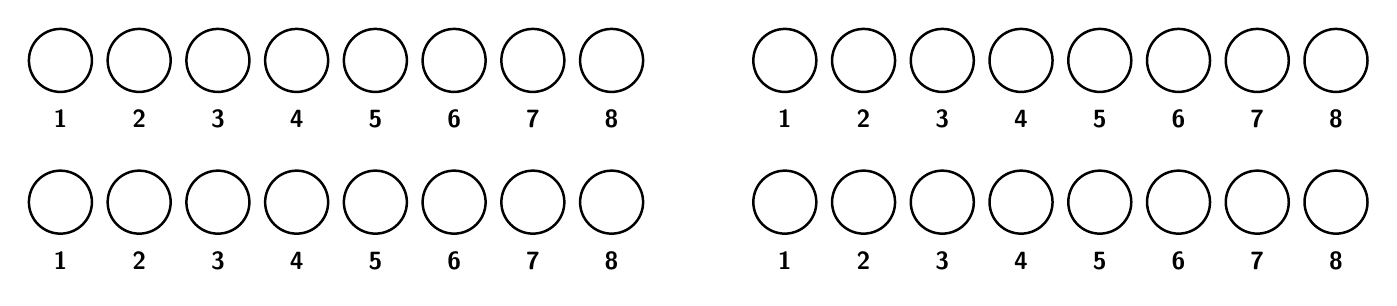
\begin{tikzpicture}
\draw[line width=0.9pt] (0.400,0.400) circle (0.400);
\node[font=\small\bfseries, anchor=base] at (0.400,-0.450) {1};
\draw[line width=0.9pt] (1.400,0.400) circle (0.400);
\node[font=\small\bfseries, anchor=base] at (1.400,-0.450) {2};
\draw[line width=0.9pt] (2.400,0.400) circle (0.400);
\node[font=\small\bfseries, anchor=base] at (2.400,-0.450) {3};
\draw[line width=0.9pt] (3.400,0.400) circle (0.400);
\node[font=\small\bfseries, anchor=base] at (3.400,-0.450) {4};
\draw[line width=0.9pt] (4.400,0.400) circle (0.400);
\node[font=\small\bfseries, anchor=base] at (4.400,-0.450) {5};
\draw[line width=0.9pt] (5.400,0.400) circle (0.400);
\node[font=\small\bfseries, anchor=base] at (5.400,-0.450) {6};
\draw[line width=0.9pt] (6.400,0.400) circle (0.400);
\node[font=\small\bfseries, anchor=base] at (6.400,-0.450) {7};
\draw[line width=0.9pt] (7.400,0.400) circle (0.400);
\node[font=\small\bfseries, anchor=base] at (7.400,-0.450) {8};
\draw[line width=0.9pt] (9.600,0.400) circle (0.400);
\node[font=\small\bfseries, anchor=base] at (9.600,-0.450) {1};
\draw[line width=0.9pt] (10.600,0.400) circle (0.400);
\node[font=\small\bfseries, anchor=base] at (10.600,-0.450) {2};
\draw[line width=0.9pt] (11.600,0.400) circle (0.400);
\node[font=\small\bfseries, anchor=base] at (11.600,-0.450) {3};
\draw[line width=0.9pt] (12.600,0.400) circle (0.400);
\node[font=\small\bfseries, anchor=base] at (12.600,-0.450) {4};
\draw[line width=0.9pt] (13.600,0.400) circle (0.400);
\node[font=\small\bfseries, anchor=base] at (13.600,-0.450) {5};
\draw[line width=0.9pt] (14.600,0.400) circle (0.400);
\node[font=\small\bfseries, anchor=base] at (14.600,-0.450) {6};
\draw[line width=0.9pt] (15.600,0.400) circle (0.400);
\node[font=\small\bfseries, anchor=base] at (15.600,-0.450) {7};
\draw[line width=0.9pt] (16.600,0.400) circle (0.400);
\node[font=\small\bfseries, anchor=base] at (16.600,-0.450) {8};
\draw[line width=0.9pt] (0.400,-1.400) circle (0.400);
\node[font=\small\bfseries, anchor=base] at (0.400,-2.250) {1};
\draw[line width=0.9pt] (1.400,-1.400) circle (0.400);
\node[font=\small\bfseries, anchor=base] at (1.400,-2.250) {2};
\draw[line width=0.9pt] (2.400,-1.400) circle (0.400);
\node[font=\small\bfseries, anchor=base] at (2.400,-2.250) {3};
\draw[line width=0.9pt] (3.400,-1.400) circle (0.400);
\node[font=\small\bfseries, anchor=base] at (3.400,-2.250) {4};
\draw[line width=0.9pt] (4.400,-1.400) circle (0.400);
\node[font=\small\bfseries, anchor=base] at (4.400,-2.250) {5};
\draw[line width=0.9pt] (5.400,-1.400) circle (0.400);
\node[font=\small\bfseries, anchor=base] at (5.400,-2.250) {6};
\draw[line width=0.9pt] (6.400,-1.400) circle (0.400);
\node[font=\small\bfseries, anchor=base] at (6.400,-2.250) {7};
\draw[line width=0.9pt] (7.400,-1.400) circle (0.400);
\node[font=\small\bfseries, anchor=base] at (7.400,-2.250) {8};
\draw[line width=0.9pt] (9.600,-1.400) circle (0.400);
\node[font=\small\bfseries, anchor=base] at (9.600,-2.250) {1};
\draw[line width=0.9pt] (10.600,-1.400) circle (0.400);
\node[font=\small\bfseries, anchor=base] at (10.600,-2.250) {2};
\draw[line width=0.9pt] (11.600,-1.400) circle (0.400);
\node[font=\small\bfseries, anchor=base] at (11.600,-2.250) {3};
\draw[line width=0.9pt] (12.600,-1.400) circle (0.400);
\node[font=\small\bfseries, anchor=base] at (12.600,-2.250) {4};
\draw[line width=0.9pt] (13.600,-1.400) circle (0.400);
\node[font=\small\bfseries, anchor=base] at (13.600,-2.250) {5};
\draw[line width=0.9pt] (14.600,-1.400) circle (0.400);
\node[font=\small\bfseries, anchor=base] at (14.600,-2.250) {6};
\draw[line width=0.9pt] (15.600,-1.400) circle (0.400);
\node[font=\small\bfseries, anchor=base] at (15.600,-2.250) {7};
\draw[line width=0.9pt] (16.600,-1.400) circle (0.400);
\node[font=\small\bfseries, anchor=base] at (16.600,-2.250) {8};
\end{tikzpicture}
\end{center}
\newpage
\par\noindent\begin{minipage}[t]{0.76\linewidth}\raggedright\textbf{Problem 5:} Color the ten lines joining five dots red or blue so that no three dots are joined by three lines of the same color. Find every way to do this.\end{minipage}\hfill\begin{minipage}[t]{0.22\linewidth}\raggedleft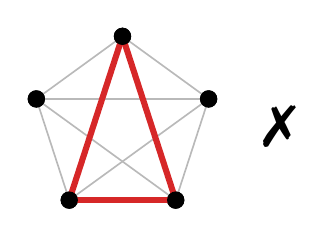
\begin{tikzpicture}[baseline=(current bounding box.north)]\draw[gray!55, line width=0.6pt] (0.000,1.150) -- (-1.094,0.355);
\draw[gray!55, line width=0.6pt] (0.000,1.150) -- (-0.676,-0.930);
\draw[gray!55, line width=0.6pt] (0.000,1.150) -- (0.676,-0.930);
\draw[gray!55, line width=0.6pt] (0.000,1.150) -- (1.094,0.355);
\draw[gray!55, line width=0.6pt] (-1.094,0.355) -- (-0.676,-0.930);
\draw[gray!55, line width=0.6pt] (-1.094,0.355) -- (0.676,-0.930);
\draw[gray!55, line width=0.6pt] (-1.094,0.355) -- (1.094,0.355);
\draw[gray!55, line width=0.6pt] (-0.676,-0.930) -- (0.676,-0.930);
\draw[gray!55, line width=0.6pt] (-0.676,-0.930) -- (1.094,0.355);
\draw[gray!55, line width=0.6pt] (0.676,-0.930) -- (1.094,0.355);
\fill (0.000,1.150) circle (0.11);
\fill (-1.094,0.355) circle (0.11);
\fill (-0.676,-0.930) circle (0.11);
\fill (0.676,-0.930) circle (0.11);
\fill (1.094,0.355) circle (0.11);
\draw[cred, line width=2.2pt] (0.000,1.150) -- (-0.676,-0.930);
\draw[cred, line width=2.2pt] (0.000,1.150) -- (0.676,-0.930);
\draw[cred, line width=2.2pt] (-0.676,-0.930) -- (0.676,-0.930);
\fill (0.000,1.150) circle (0.11);
\fill (-1.094,0.355) circle (0.11);
\fill (-0.676,-0.930) circle (0.11);
\fill (0.676,-0.930) circle (0.11);
\fill (1.094,0.355) circle (0.11);
\node[font=\huge] at (2.000,0) {\ding{55}};\end{tikzpicture}\end{minipage}\par

\vspace{2pt}\begin{center}
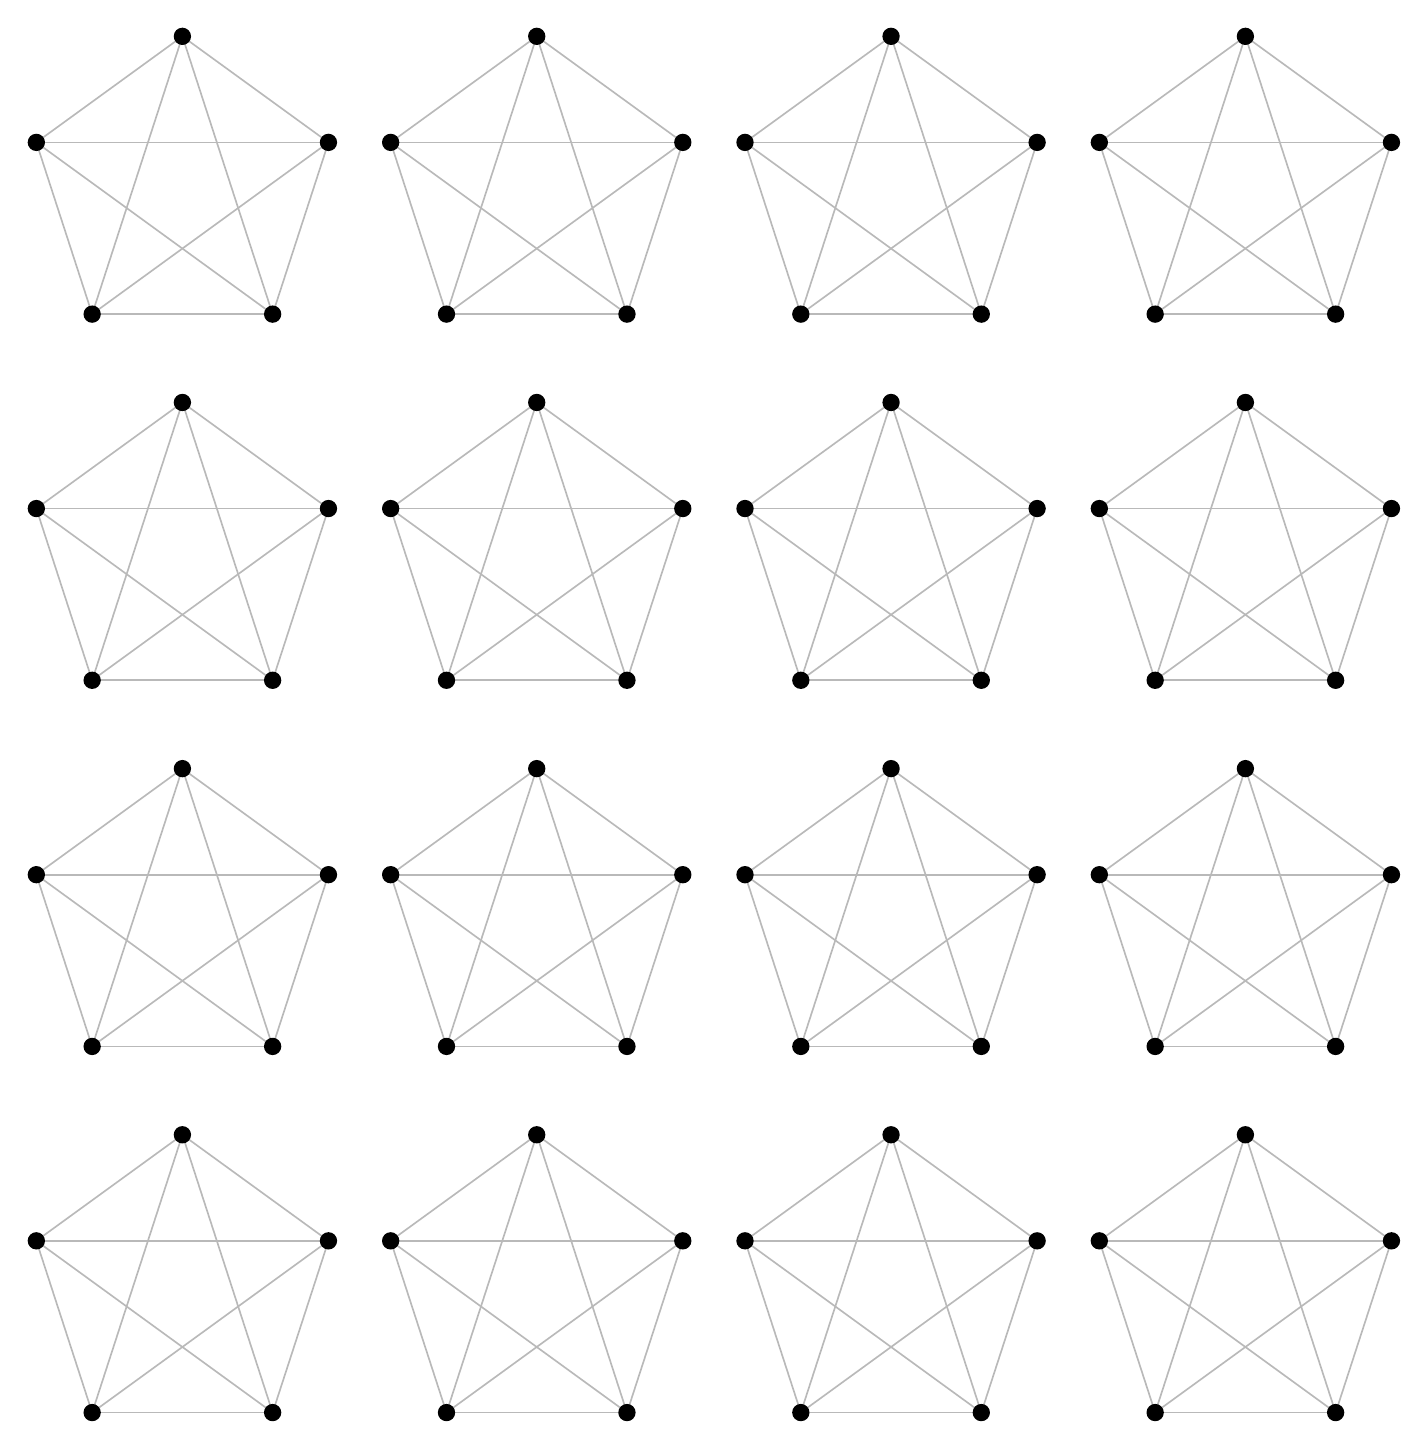
\begin{tikzpicture}
\draw[gray!55, line width=0.6pt] (0.000,1.950) -- (-1.855,0.603);
\draw[gray!55, line width=0.6pt] (0.000,1.950) -- (-1.146,-1.578);
\draw[gray!55, line width=0.6pt] (0.000,1.950) -- (1.146,-1.578);
\draw[gray!55, line width=0.6pt] (0.000,1.950) -- (1.855,0.603);
\draw[gray!55, line width=0.6pt] (-1.855,0.603) -- (-1.146,-1.578);
\draw[gray!55, line width=0.6pt] (-1.855,0.603) -- (1.146,-1.578);
\draw[gray!55, line width=0.6pt] (-1.855,0.603) -- (1.855,0.603);
\draw[gray!55, line width=0.6pt] (-1.146,-1.578) -- (1.146,-1.578);
\draw[gray!55, line width=0.6pt] (-1.146,-1.578) -- (1.855,0.603);
\draw[gray!55, line width=0.6pt] (1.146,-1.578) -- (1.855,0.603);
\fill (0.000,1.950) circle (0.11);
\fill (-1.855,0.603) circle (0.11);
\fill (-1.146,-1.578) circle (0.11);
\fill (1.146,-1.578) circle (0.11);
\fill (1.855,0.603) circle (0.11);
\draw[gray!55, line width=0.6pt] (4.500,1.950) -- (2.645,0.603);
\draw[gray!55, line width=0.6pt] (4.500,1.950) -- (3.354,-1.578);
\draw[gray!55, line width=0.6pt] (4.500,1.950) -- (5.646,-1.578);
\draw[gray!55, line width=0.6pt] (4.500,1.950) -- (6.355,0.603);
\draw[gray!55, line width=0.6pt] (2.645,0.603) -- (3.354,-1.578);
\draw[gray!55, line width=0.6pt] (2.645,0.603) -- (5.646,-1.578);
\draw[gray!55, line width=0.6pt] (2.645,0.603) -- (6.355,0.603);
\draw[gray!55, line width=0.6pt] (3.354,-1.578) -- (5.646,-1.578);
\draw[gray!55, line width=0.6pt] (3.354,-1.578) -- (6.355,0.603);
\draw[gray!55, line width=0.6pt] (5.646,-1.578) -- (6.355,0.603);
\fill (4.500,1.950) circle (0.11);
\fill (2.645,0.603) circle (0.11);
\fill (3.354,-1.578) circle (0.11);
\fill (5.646,-1.578) circle (0.11);
\fill (6.355,0.603) circle (0.11);
\draw[gray!55, line width=0.6pt] (9.000,1.950) -- (7.145,0.603);
\draw[gray!55, line width=0.6pt] (9.000,1.950) -- (7.854,-1.578);
\draw[gray!55, line width=0.6pt] (9.000,1.950) -- (10.146,-1.578);
\draw[gray!55, line width=0.6pt] (9.000,1.950) -- (10.855,0.603);
\draw[gray!55, line width=0.6pt] (7.145,0.603) -- (7.854,-1.578);
\draw[gray!55, line width=0.6pt] (7.145,0.603) -- (10.146,-1.578);
\draw[gray!55, line width=0.6pt] (7.145,0.603) -- (10.855,0.603);
\draw[gray!55, line width=0.6pt] (7.854,-1.578) -- (10.146,-1.578);
\draw[gray!55, line width=0.6pt] (7.854,-1.578) -- (10.855,0.603);
\draw[gray!55, line width=0.6pt] (10.146,-1.578) -- (10.855,0.603);
\fill (9.000,1.950) circle (0.11);
\fill (7.145,0.603) circle (0.11);
\fill (7.854,-1.578) circle (0.11);
\fill (10.146,-1.578) circle (0.11);
\fill (10.855,0.603) circle (0.11);
\draw[gray!55, line width=0.6pt] (13.500,1.950) -- (11.645,0.603);
\draw[gray!55, line width=0.6pt] (13.500,1.950) -- (12.354,-1.578);
\draw[gray!55, line width=0.6pt] (13.500,1.950) -- (14.646,-1.578);
\draw[gray!55, line width=0.6pt] (13.500,1.950) -- (15.355,0.603);
\draw[gray!55, line width=0.6pt] (11.645,0.603) -- (12.354,-1.578);
\draw[gray!55, line width=0.6pt] (11.645,0.603) -- (14.646,-1.578);
\draw[gray!55, line width=0.6pt] (11.645,0.603) -- (15.355,0.603);
\draw[gray!55, line width=0.6pt] (12.354,-1.578) -- (14.646,-1.578);
\draw[gray!55, line width=0.6pt] (12.354,-1.578) -- (15.355,0.603);
\draw[gray!55, line width=0.6pt] (14.646,-1.578) -- (15.355,0.603);
\fill (13.500,1.950) circle (0.11);
\fill (11.645,0.603) circle (0.11);
\fill (12.354,-1.578) circle (0.11);
\fill (14.646,-1.578) circle (0.11);
\fill (15.355,0.603) circle (0.11);
\draw[gray!55, line width=0.6pt] (0.000,-2.700) -- (-1.855,-4.047);
\draw[gray!55, line width=0.6pt] (0.000,-2.700) -- (-1.146,-6.228);
\draw[gray!55, line width=0.6pt] (0.000,-2.700) -- (1.146,-6.228);
\draw[gray!55, line width=0.6pt] (0.000,-2.700) -- (1.855,-4.047);
\draw[gray!55, line width=0.6pt] (-1.855,-4.047) -- (-1.146,-6.228);
\draw[gray!55, line width=0.6pt] (-1.855,-4.047) -- (1.146,-6.228);
\draw[gray!55, line width=0.6pt] (-1.855,-4.047) -- (1.855,-4.047);
\draw[gray!55, line width=0.6pt] (-1.146,-6.228) -- (1.146,-6.228);
\draw[gray!55, line width=0.6pt] (-1.146,-6.228) -- (1.855,-4.047);
\draw[gray!55, line width=0.6pt] (1.146,-6.228) -- (1.855,-4.047);
\fill (0.000,-2.700) circle (0.11);
\fill (-1.855,-4.047) circle (0.11);
\fill (-1.146,-6.228) circle (0.11);
\fill (1.146,-6.228) circle (0.11);
\fill (1.855,-4.047) circle (0.11);
\draw[gray!55, line width=0.6pt] (4.500,-2.700) -- (2.645,-4.047);
\draw[gray!55, line width=0.6pt] (4.500,-2.700) -- (3.354,-6.228);
\draw[gray!55, line width=0.6pt] (4.500,-2.700) -- (5.646,-6.228);
\draw[gray!55, line width=0.6pt] (4.500,-2.700) -- (6.355,-4.047);
\draw[gray!55, line width=0.6pt] (2.645,-4.047) -- (3.354,-6.228);
\draw[gray!55, line width=0.6pt] (2.645,-4.047) -- (5.646,-6.228);
\draw[gray!55, line width=0.6pt] (2.645,-4.047) -- (6.355,-4.047);
\draw[gray!55, line width=0.6pt] (3.354,-6.228) -- (5.646,-6.228);
\draw[gray!55, line width=0.6pt] (3.354,-6.228) -- (6.355,-4.047);
\draw[gray!55, line width=0.6pt] (5.646,-6.228) -- (6.355,-4.047);
\fill (4.500,-2.700) circle (0.11);
\fill (2.645,-4.047) circle (0.11);
\fill (3.354,-6.228) circle (0.11);
\fill (5.646,-6.228) circle (0.11);
\fill (6.355,-4.047) circle (0.11);
\draw[gray!55, line width=0.6pt] (9.000,-2.700) -- (7.145,-4.047);
\draw[gray!55, line width=0.6pt] (9.000,-2.700) -- (7.854,-6.228);
\draw[gray!55, line width=0.6pt] (9.000,-2.700) -- (10.146,-6.228);
\draw[gray!55, line width=0.6pt] (9.000,-2.700) -- (10.855,-4.047);
\draw[gray!55, line width=0.6pt] (7.145,-4.047) -- (7.854,-6.228);
\draw[gray!55, line width=0.6pt] (7.145,-4.047) -- (10.146,-6.228);
\draw[gray!55, line width=0.6pt] (7.145,-4.047) -- (10.855,-4.047);
\draw[gray!55, line width=0.6pt] (7.854,-6.228) -- (10.146,-6.228);
\draw[gray!55, line width=0.6pt] (7.854,-6.228) -- (10.855,-4.047);
\draw[gray!55, line width=0.6pt] (10.146,-6.228) -- (10.855,-4.047);
\fill (9.000,-2.700) circle (0.11);
\fill (7.145,-4.047) circle (0.11);
\fill (7.854,-6.228) circle (0.11);
\fill (10.146,-6.228) circle (0.11);
\fill (10.855,-4.047) circle (0.11);
\draw[gray!55, line width=0.6pt] (13.500,-2.700) -- (11.645,-4.047);
\draw[gray!55, line width=0.6pt] (13.500,-2.700) -- (12.354,-6.228);
\draw[gray!55, line width=0.6pt] (13.500,-2.700) -- (14.646,-6.228);
\draw[gray!55, line width=0.6pt] (13.500,-2.700) -- (15.355,-4.047);
\draw[gray!55, line width=0.6pt] (11.645,-4.047) -- (12.354,-6.228);
\draw[gray!55, line width=0.6pt] (11.645,-4.047) -- (14.646,-6.228);
\draw[gray!55, line width=0.6pt] (11.645,-4.047) -- (15.355,-4.047);
\draw[gray!55, line width=0.6pt] (12.354,-6.228) -- (14.646,-6.228);
\draw[gray!55, line width=0.6pt] (12.354,-6.228) -- (15.355,-4.047);
\draw[gray!55, line width=0.6pt] (14.646,-6.228) -- (15.355,-4.047);
\fill (13.500,-2.700) circle (0.11);
\fill (11.645,-4.047) circle (0.11);
\fill (12.354,-6.228) circle (0.11);
\fill (14.646,-6.228) circle (0.11);
\fill (15.355,-4.047) circle (0.11);
\draw[gray!55, line width=0.6pt] (0.000,-7.350) -- (-1.855,-8.697);
\draw[gray!55, line width=0.6pt] (0.000,-7.350) -- (-1.146,-10.878);
\draw[gray!55, line width=0.6pt] (0.000,-7.350) -- (1.146,-10.878);
\draw[gray!55, line width=0.6pt] (0.000,-7.350) -- (1.855,-8.697);
\draw[gray!55, line width=0.6pt] (-1.855,-8.697) -- (-1.146,-10.878);
\draw[gray!55, line width=0.6pt] (-1.855,-8.697) -- (1.146,-10.878);
\draw[gray!55, line width=0.6pt] (-1.855,-8.697) -- (1.855,-8.697);
\draw[gray!55, line width=0.6pt] (-1.146,-10.878) -- (1.146,-10.878);
\draw[gray!55, line width=0.6pt] (-1.146,-10.878) -- (1.855,-8.697);
\draw[gray!55, line width=0.6pt] (1.146,-10.878) -- (1.855,-8.697);
\fill (0.000,-7.350) circle (0.11);
\fill (-1.855,-8.697) circle (0.11);
\fill (-1.146,-10.878) circle (0.11);
\fill (1.146,-10.878) circle (0.11);
\fill (1.855,-8.697) circle (0.11);
\draw[gray!55, line width=0.6pt] (4.500,-7.350) -- (2.645,-8.697);
\draw[gray!55, line width=0.6pt] (4.500,-7.350) -- (3.354,-10.878);
\draw[gray!55, line width=0.6pt] (4.500,-7.350) -- (5.646,-10.878);
\draw[gray!55, line width=0.6pt] (4.500,-7.350) -- (6.355,-8.697);
\draw[gray!55, line width=0.6pt] (2.645,-8.697) -- (3.354,-10.878);
\draw[gray!55, line width=0.6pt] (2.645,-8.697) -- (5.646,-10.878);
\draw[gray!55, line width=0.6pt] (2.645,-8.697) -- (6.355,-8.697);
\draw[gray!55, line width=0.6pt] (3.354,-10.878) -- (5.646,-10.878);
\draw[gray!55, line width=0.6pt] (3.354,-10.878) -- (6.355,-8.697);
\draw[gray!55, line width=0.6pt] (5.646,-10.878) -- (6.355,-8.697);
\fill (4.500,-7.350) circle (0.11);
\fill (2.645,-8.697) circle (0.11);
\fill (3.354,-10.878) circle (0.11);
\fill (5.646,-10.878) circle (0.11);
\fill (6.355,-8.697) circle (0.11);
\draw[gray!55, line width=0.6pt] (9.000,-7.350) -- (7.145,-8.697);
\draw[gray!55, line width=0.6pt] (9.000,-7.350) -- (7.854,-10.878);
\draw[gray!55, line width=0.6pt] (9.000,-7.350) -- (10.146,-10.878);
\draw[gray!55, line width=0.6pt] (9.000,-7.350) -- (10.855,-8.697);
\draw[gray!55, line width=0.6pt] (7.145,-8.697) -- (7.854,-10.878);
\draw[gray!55, line width=0.6pt] (7.145,-8.697) -- (10.146,-10.878);
\draw[gray!55, line width=0.6pt] (7.145,-8.697) -- (10.855,-8.697);
\draw[gray!55, line width=0.6pt] (7.854,-10.878) -- (10.146,-10.878);
\draw[gray!55, line width=0.6pt] (7.854,-10.878) -- (10.855,-8.697);
\draw[gray!55, line width=0.6pt] (10.146,-10.878) -- (10.855,-8.697);
\fill (9.000,-7.350) circle (0.11);
\fill (7.145,-8.697) circle (0.11);
\fill (7.854,-10.878) circle (0.11);
\fill (10.146,-10.878) circle (0.11);
\fill (10.855,-8.697) circle (0.11);
\draw[gray!55, line width=0.6pt] (13.500,-7.350) -- (11.645,-8.697);
\draw[gray!55, line width=0.6pt] (13.500,-7.350) -- (12.354,-10.878);
\draw[gray!55, line width=0.6pt] (13.500,-7.350) -- (14.646,-10.878);
\draw[gray!55, line width=0.6pt] (13.500,-7.350) -- (15.355,-8.697);
\draw[gray!55, line width=0.6pt] (11.645,-8.697) -- (12.354,-10.878);
\draw[gray!55, line width=0.6pt] (11.645,-8.697) -- (14.646,-10.878);
\draw[gray!55, line width=0.6pt] (11.645,-8.697) -- (15.355,-8.697);
\draw[gray!55, line width=0.6pt] (12.354,-10.878) -- (14.646,-10.878);
\draw[gray!55, line width=0.6pt] (12.354,-10.878) -- (15.355,-8.697);
\draw[gray!55, line width=0.6pt] (14.646,-10.878) -- (15.355,-8.697);
\fill (13.500,-7.350) circle (0.11);
\fill (11.645,-8.697) circle (0.11);
\fill (12.354,-10.878) circle (0.11);
\fill (14.646,-10.878) circle (0.11);
\fill (15.355,-8.697) circle (0.11);
\draw[gray!55, line width=0.6pt] (0.000,-12.000) -- (-1.855,-13.347);
\draw[gray!55, line width=0.6pt] (0.000,-12.000) -- (-1.146,-15.528);
\draw[gray!55, line width=0.6pt] (0.000,-12.000) -- (1.146,-15.528);
\draw[gray!55, line width=0.6pt] (0.000,-12.000) -- (1.855,-13.347);
\draw[gray!55, line width=0.6pt] (-1.855,-13.347) -- (-1.146,-15.528);
\draw[gray!55, line width=0.6pt] (-1.855,-13.347) -- (1.146,-15.528);
\draw[gray!55, line width=0.6pt] (-1.855,-13.347) -- (1.855,-13.347);
\draw[gray!55, line width=0.6pt] (-1.146,-15.528) -- (1.146,-15.528);
\draw[gray!55, line width=0.6pt] (-1.146,-15.528) -- (1.855,-13.347);
\draw[gray!55, line width=0.6pt] (1.146,-15.528) -- (1.855,-13.347);
\fill (0.000,-12.000) circle (0.11);
\fill (-1.855,-13.347) circle (0.11);
\fill (-1.146,-15.528) circle (0.11);
\fill (1.146,-15.528) circle (0.11);
\fill (1.855,-13.347) circle (0.11);
\draw[gray!55, line width=0.6pt] (4.500,-12.000) -- (2.645,-13.347);
\draw[gray!55, line width=0.6pt] (4.500,-12.000) -- (3.354,-15.528);
\draw[gray!55, line width=0.6pt] (4.500,-12.000) -- (5.646,-15.528);
\draw[gray!55, line width=0.6pt] (4.500,-12.000) -- (6.355,-13.347);
\draw[gray!55, line width=0.6pt] (2.645,-13.347) -- (3.354,-15.528);
\draw[gray!55, line width=0.6pt] (2.645,-13.347) -- (5.646,-15.528);
\draw[gray!55, line width=0.6pt] (2.645,-13.347) -- (6.355,-13.347);
\draw[gray!55, line width=0.6pt] (3.354,-15.528) -- (5.646,-15.528);
\draw[gray!55, line width=0.6pt] (3.354,-15.528) -- (6.355,-13.347);
\draw[gray!55, line width=0.6pt] (5.646,-15.528) -- (6.355,-13.347);
\fill (4.500,-12.000) circle (0.11);
\fill (2.645,-13.347) circle (0.11);
\fill (3.354,-15.528) circle (0.11);
\fill (5.646,-15.528) circle (0.11);
\fill (6.355,-13.347) circle (0.11);
\draw[gray!55, line width=0.6pt] (9.000,-12.000) -- (7.145,-13.347);
\draw[gray!55, line width=0.6pt] (9.000,-12.000) -- (7.854,-15.528);
\draw[gray!55, line width=0.6pt] (9.000,-12.000) -- (10.146,-15.528);
\draw[gray!55, line width=0.6pt] (9.000,-12.000) -- (10.855,-13.347);
\draw[gray!55, line width=0.6pt] (7.145,-13.347) -- (7.854,-15.528);
\draw[gray!55, line width=0.6pt] (7.145,-13.347) -- (10.146,-15.528);
\draw[gray!55, line width=0.6pt] (7.145,-13.347) -- (10.855,-13.347);
\draw[gray!55, line width=0.6pt] (7.854,-15.528) -- (10.146,-15.528);
\draw[gray!55, line width=0.6pt] (7.854,-15.528) -- (10.855,-13.347);
\draw[gray!55, line width=0.6pt] (10.146,-15.528) -- (10.855,-13.347);
\fill (9.000,-12.000) circle (0.11);
\fill (7.145,-13.347) circle (0.11);
\fill (7.854,-15.528) circle (0.11);
\fill (10.146,-15.528) circle (0.11);
\fill (10.855,-13.347) circle (0.11);
\draw[gray!55, line width=0.6pt] (13.500,-12.000) -- (11.645,-13.347);
\draw[gray!55, line width=0.6pt] (13.500,-12.000) -- (12.354,-15.528);
\draw[gray!55, line width=0.6pt] (13.500,-12.000) -- (14.646,-15.528);
\draw[gray!55, line width=0.6pt] (13.500,-12.000) -- (15.355,-13.347);
\draw[gray!55, line width=0.6pt] (11.645,-13.347) -- (12.354,-15.528);
\draw[gray!55, line width=0.6pt] (11.645,-13.347) -- (14.646,-15.528);
\draw[gray!55, line width=0.6pt] (11.645,-13.347) -- (15.355,-13.347);
\draw[gray!55, line width=0.6pt] (12.354,-15.528) -- (14.646,-15.528);
\draw[gray!55, line width=0.6pt] (12.354,-15.528) -- (15.355,-13.347);
\draw[gray!55, line width=0.6pt] (14.646,-15.528) -- (15.355,-13.347);
\fill (13.500,-12.000) circle (0.11);
\fill (11.645,-13.347) circle (0.11);
\fill (12.354,-15.528) circle (0.11);
\fill (14.646,-15.528) circle (0.11);
\fill (15.355,-13.347) circle (0.11);
\end{tikzpicture}
\end{center}
\newpage
\par\noindent\textbf{Problem 6:} Play Sim with a partner on a board of six dots. One player colors lines red and the other blue. Take turns, coloring one line each turn. If you join three dots with three lines of your own color, you lose. Would you rather go first or second?\par

\vspace{4pt}\begin{center}
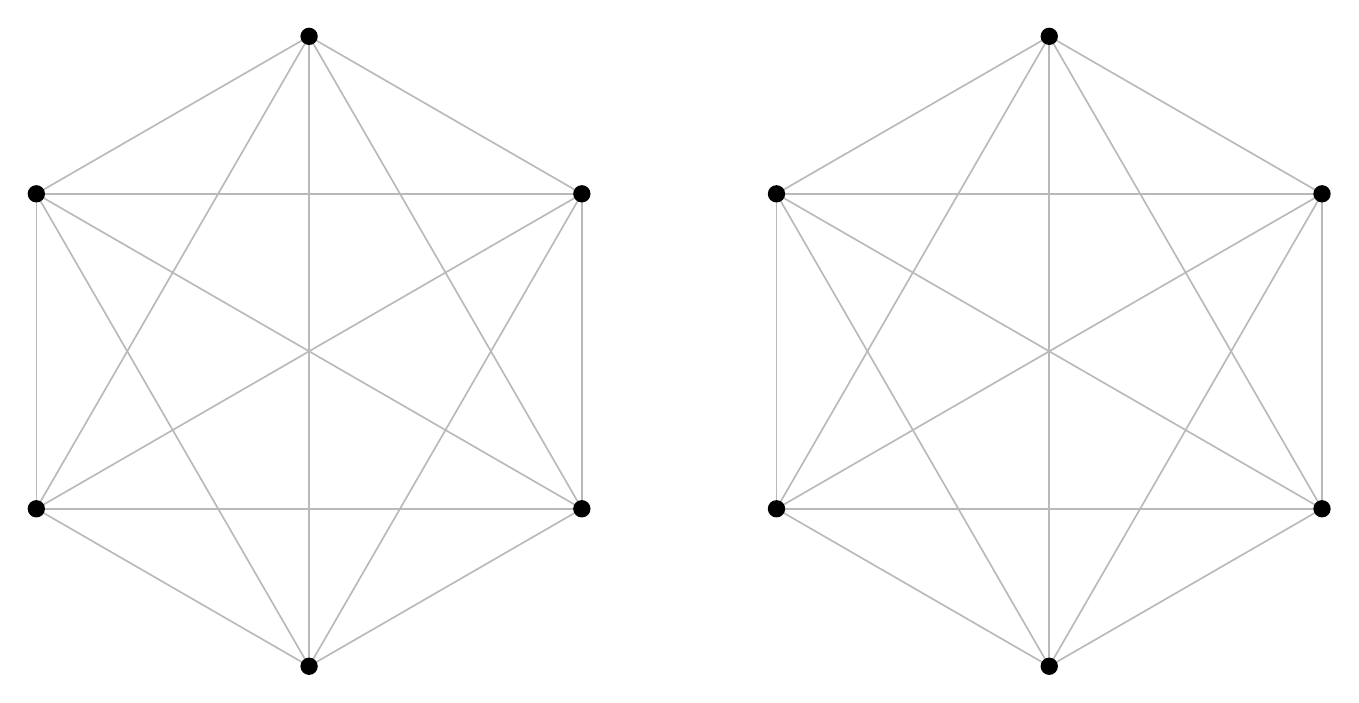
\begin{tikzpicture}
\draw[gray!55, line width=0.6pt] (0.000,4.000) -- (-3.464,2.000);
\draw[gray!55, line width=0.6pt] (0.000,4.000) -- (-3.464,-2.000);
\draw[gray!55, line width=0.6pt] (0.000,4.000) -- (-0.000,-4.000);
\draw[gray!55, line width=0.6pt] (0.000,4.000) -- (3.464,-2.000);
\draw[gray!55, line width=0.6pt] (0.000,4.000) -- (3.464,2.000);
\draw[gray!55, line width=0.6pt] (-3.464,2.000) -- (-3.464,-2.000);
\draw[gray!55, line width=0.6pt] (-3.464,2.000) -- (-0.000,-4.000);
\draw[gray!55, line width=0.6pt] (-3.464,2.000) -- (3.464,-2.000);
\draw[gray!55, line width=0.6pt] (-3.464,2.000) -- (3.464,2.000);
\draw[gray!55, line width=0.6pt] (-3.464,-2.000) -- (-0.000,-4.000);
\draw[gray!55, line width=0.6pt] (-3.464,-2.000) -- (3.464,-2.000);
\draw[gray!55, line width=0.6pt] (-3.464,-2.000) -- (3.464,2.000);
\draw[gray!55, line width=0.6pt] (-0.000,-4.000) -- (3.464,-2.000);
\draw[gray!55, line width=0.6pt] (-0.000,-4.000) -- (3.464,2.000);
\draw[gray!55, line width=0.6pt] (3.464,-2.000) -- (3.464,2.000);
\fill (0.000,4.000) circle (0.11);
\fill (-3.464,2.000) circle (0.11);
\fill (-3.464,-2.000) circle (0.11);
\fill (-0.000,-4.000) circle (0.11);
\fill (3.464,-2.000) circle (0.11);
\fill (3.464,2.000) circle (0.11);
\draw[gray!55, line width=0.6pt] (9.400,4.000) -- (5.936,2.000);
\draw[gray!55, line width=0.6pt] (9.400,4.000) -- (5.936,-2.000);
\draw[gray!55, line width=0.6pt] (9.400,4.000) -- (9.400,-4.000);
\draw[gray!55, line width=0.6pt] (9.400,4.000) -- (12.864,-2.000);
\draw[gray!55, line width=0.6pt] (9.400,4.000) -- (12.864,2.000);
\draw[gray!55, line width=0.6pt] (5.936,2.000) -- (5.936,-2.000);
\draw[gray!55, line width=0.6pt] (5.936,2.000) -- (9.400,-4.000);
\draw[gray!55, line width=0.6pt] (5.936,2.000) -- (12.864,-2.000);
\draw[gray!55, line width=0.6pt] (5.936,2.000) -- (12.864,2.000);
\draw[gray!55, line width=0.6pt] (5.936,-2.000) -- (9.400,-4.000);
\draw[gray!55, line width=0.6pt] (5.936,-2.000) -- (12.864,-2.000);
\draw[gray!55, line width=0.6pt] (5.936,-2.000) -- (12.864,2.000);
\draw[gray!55, line width=0.6pt] (9.400,-4.000) -- (12.864,-2.000);
\draw[gray!55, line width=0.6pt] (9.400,-4.000) -- (12.864,2.000);
\draw[gray!55, line width=0.6pt] (12.864,-2.000) -- (12.864,2.000);
\fill (9.400,4.000) circle (0.11);
\fill (5.936,2.000) circle (0.11);
\fill (5.936,-2.000) circle (0.11);
\fill (9.400,-4.000) circle (0.11);
\fill (12.864,-2.000) circle (0.11);
\fill (12.864,2.000) circle (0.11);
\end{tikzpicture}
\end{center}
\vspace{0.4cm}
\par\noindent\textbf{Problem 7:} Can the fifteen lines joining six dots be colored red or blue with no one-color triangle (three dots joined by three lines of one color)? Explain how you know.\par

\vspace{4pt}\begin{center}
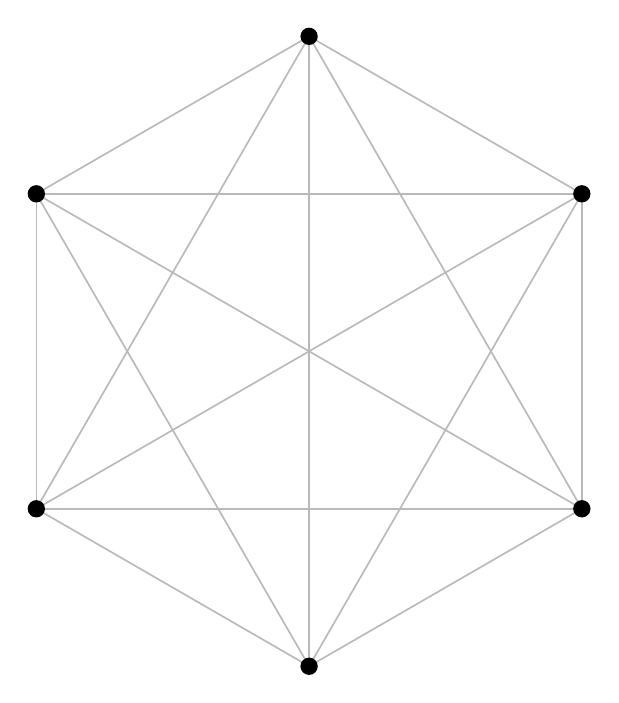
\begin{tikzpicture}
\draw[gray!55, line width=0.6pt] (0.000,4.000) -- (-3.464,2.000);
\draw[gray!55, line width=0.6pt] (0.000,4.000) -- (-3.464,-2.000);
\draw[gray!55, line width=0.6pt] (0.000,4.000) -- (-0.000,-4.000);
\draw[gray!55, line width=0.6pt] (0.000,4.000) -- (3.464,-2.000);
\draw[gray!55, line width=0.6pt] (0.000,4.000) -- (3.464,2.000);
\draw[gray!55, line width=0.6pt] (-3.464,2.000) -- (-3.464,-2.000);
\draw[gray!55, line width=0.6pt] (-3.464,2.000) -- (-0.000,-4.000);
\draw[gray!55, line width=0.6pt] (-3.464,2.000) -- (3.464,-2.000);
\draw[gray!55, line width=0.6pt] (-3.464,2.000) -- (3.464,2.000);
\draw[gray!55, line width=0.6pt] (-3.464,-2.000) -- (-0.000,-4.000);
\draw[gray!55, line width=0.6pt] (-3.464,-2.000) -- (3.464,-2.000);
\draw[gray!55, line width=0.6pt] (-3.464,-2.000) -- (3.464,2.000);
\draw[gray!55, line width=0.6pt] (-0.000,-4.000) -- (3.464,-2.000);
\draw[gray!55, line width=0.6pt] (-0.000,-4.000) -- (3.464,2.000);
\draw[gray!55, line width=0.6pt] (3.464,-2.000) -- (3.464,2.000);
\fill (0.000,4.000) circle (0.11);
\fill (-3.464,2.000) circle (0.11);
\fill (-3.464,-2.000) circle (0.11);
\fill (-0.000,-4.000) circle (0.11);
\fill (3.464,-2.000) circle (0.11);
\fill (3.464,2.000) circle (0.11);
\end{tikzpicture}
\end{center}
\newpage
\par\noindent\textbf{Problem 8:} Color the fifteen lines joining six dots red or blue with as few one-color triangles as possible. What is the fewest you can get?\par

\vspace{4pt}\begin{center}
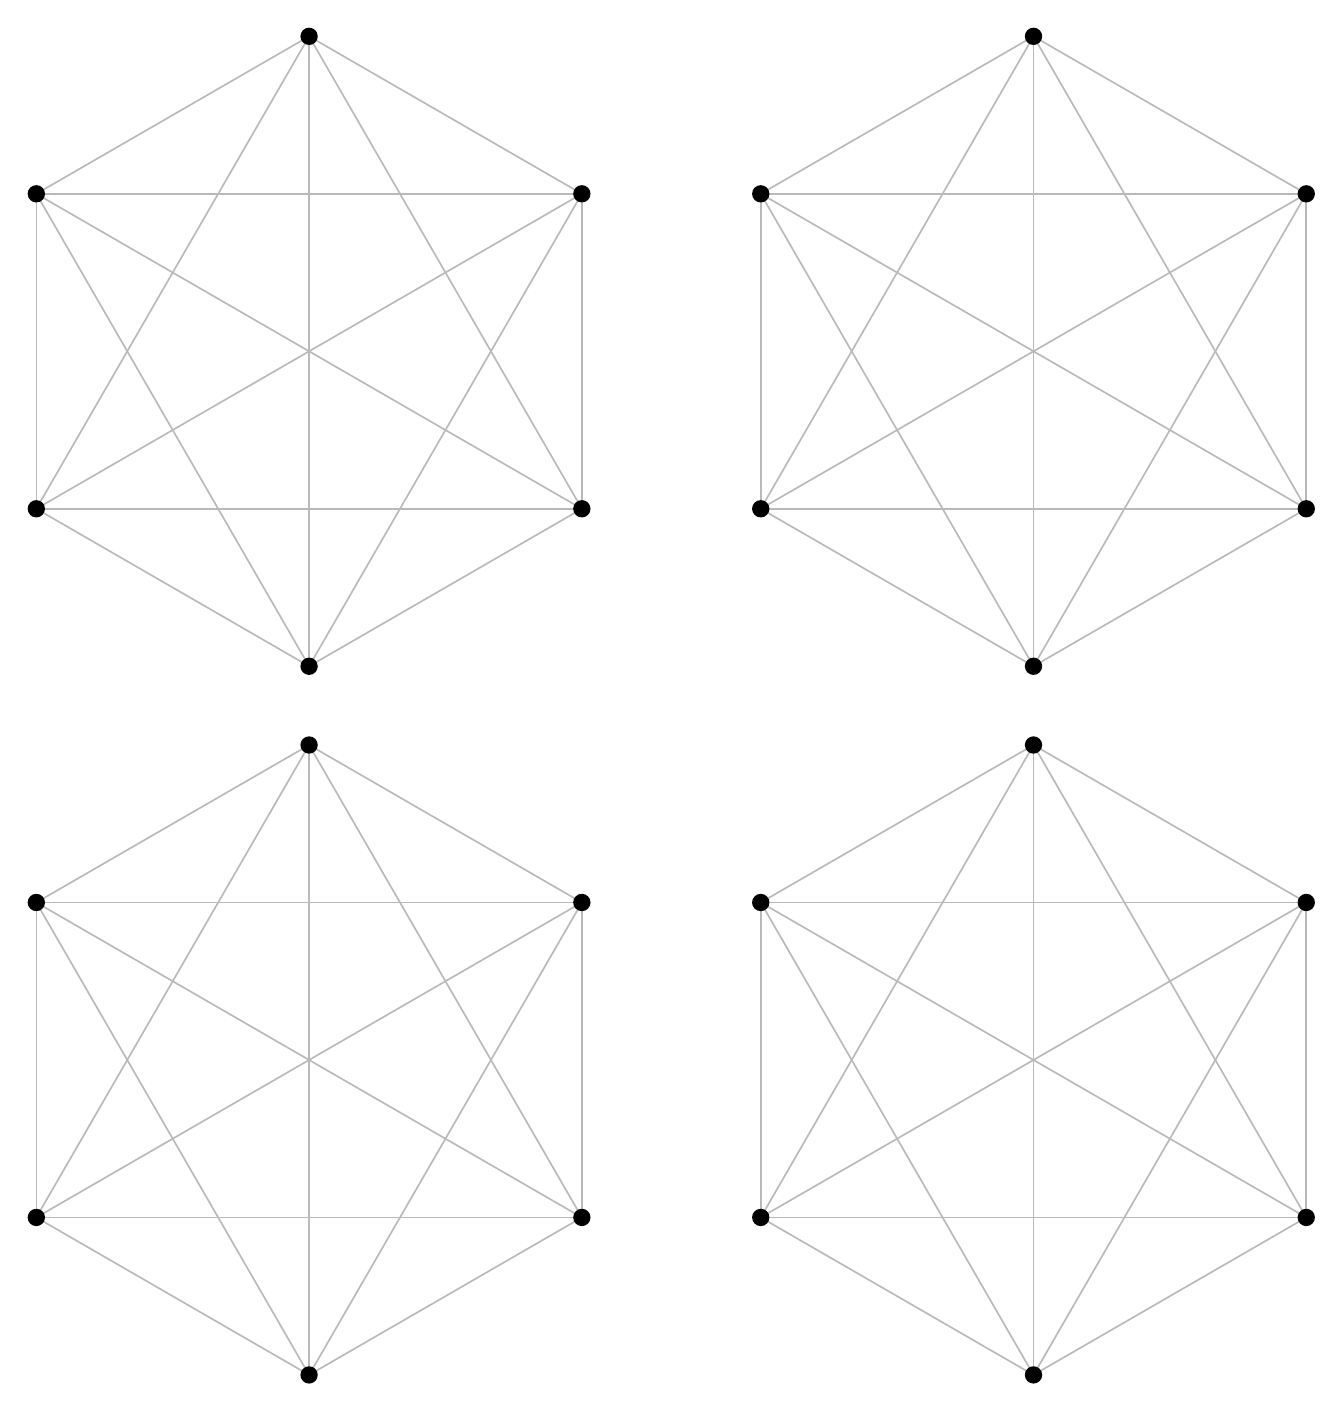
\begin{tikzpicture}
\draw[gray!55, line width=0.6pt] (0.000,4.000) -- (-3.464,2.000);
\draw[gray!55, line width=0.6pt] (0.000,4.000) -- (-3.464,-2.000);
\draw[gray!55, line width=0.6pt] (0.000,4.000) -- (-0.000,-4.000);
\draw[gray!55, line width=0.6pt] (0.000,4.000) -- (3.464,-2.000);
\draw[gray!55, line width=0.6pt] (0.000,4.000) -- (3.464,2.000);
\draw[gray!55, line width=0.6pt] (-3.464,2.000) -- (-3.464,-2.000);
\draw[gray!55, line width=0.6pt] (-3.464,2.000) -- (-0.000,-4.000);
\draw[gray!55, line width=0.6pt] (-3.464,2.000) -- (3.464,-2.000);
\draw[gray!55, line width=0.6pt] (-3.464,2.000) -- (3.464,2.000);
\draw[gray!55, line width=0.6pt] (-3.464,-2.000) -- (-0.000,-4.000);
\draw[gray!55, line width=0.6pt] (-3.464,-2.000) -- (3.464,-2.000);
\draw[gray!55, line width=0.6pt] (-3.464,-2.000) -- (3.464,2.000);
\draw[gray!55, line width=0.6pt] (-0.000,-4.000) -- (3.464,-2.000);
\draw[gray!55, line width=0.6pt] (-0.000,-4.000) -- (3.464,2.000);
\draw[gray!55, line width=0.6pt] (3.464,-2.000) -- (3.464,2.000);
\fill (0.000,4.000) circle (0.11);
\fill (-3.464,2.000) circle (0.11);
\fill (-3.464,-2.000) circle (0.11);
\fill (-0.000,-4.000) circle (0.11);
\fill (3.464,-2.000) circle (0.11);
\fill (3.464,2.000) circle (0.11);
\draw[gray!55, line width=0.6pt] (9.200,4.000) -- (5.736,2.000);
\draw[gray!55, line width=0.6pt] (9.200,4.000) -- (5.736,-2.000);
\draw[gray!55, line width=0.6pt] (9.200,4.000) -- (9.200,-4.000);
\draw[gray!55, line width=0.6pt] (9.200,4.000) -- (12.664,-2.000);
\draw[gray!55, line width=0.6pt] (9.200,4.000) -- (12.664,2.000);
\draw[gray!55, line width=0.6pt] (5.736,2.000) -- (5.736,-2.000);
\draw[gray!55, line width=0.6pt] (5.736,2.000) -- (9.200,-4.000);
\draw[gray!55, line width=0.6pt] (5.736,2.000) -- (12.664,-2.000);
\draw[gray!55, line width=0.6pt] (5.736,2.000) -- (12.664,2.000);
\draw[gray!55, line width=0.6pt] (5.736,-2.000) -- (9.200,-4.000);
\draw[gray!55, line width=0.6pt] (5.736,-2.000) -- (12.664,-2.000);
\draw[gray!55, line width=0.6pt] (5.736,-2.000) -- (12.664,2.000);
\draw[gray!55, line width=0.6pt] (9.200,-4.000) -- (12.664,-2.000);
\draw[gray!55, line width=0.6pt] (9.200,-4.000) -- (12.664,2.000);
\draw[gray!55, line width=0.6pt] (12.664,-2.000) -- (12.664,2.000);
\fill (9.200,4.000) circle (0.11);
\fill (5.736,2.000) circle (0.11);
\fill (5.736,-2.000) circle (0.11);
\fill (9.200,-4.000) circle (0.11);
\fill (12.664,-2.000) circle (0.11);
\fill (12.664,2.000) circle (0.11);
\draw[gray!55, line width=0.6pt] (0.000,-5.000) -- (-3.464,-7.000);
\draw[gray!55, line width=0.6pt] (0.000,-5.000) -- (-3.464,-11.000);
\draw[gray!55, line width=0.6pt] (0.000,-5.000) -- (-0.000,-13.000);
\draw[gray!55, line width=0.6pt] (0.000,-5.000) -- (3.464,-11.000);
\draw[gray!55, line width=0.6pt] (0.000,-5.000) -- (3.464,-7.000);
\draw[gray!55, line width=0.6pt] (-3.464,-7.000) -- (-3.464,-11.000);
\draw[gray!55, line width=0.6pt] (-3.464,-7.000) -- (-0.000,-13.000);
\draw[gray!55, line width=0.6pt] (-3.464,-7.000) -- (3.464,-11.000);
\draw[gray!55, line width=0.6pt] (-3.464,-7.000) -- (3.464,-7.000);
\draw[gray!55, line width=0.6pt] (-3.464,-11.000) -- (-0.000,-13.000);
\draw[gray!55, line width=0.6pt] (-3.464,-11.000) -- (3.464,-11.000);
\draw[gray!55, line width=0.6pt] (-3.464,-11.000) -- (3.464,-7.000);
\draw[gray!55, line width=0.6pt] (-0.000,-13.000) -- (3.464,-11.000);
\draw[gray!55, line width=0.6pt] (-0.000,-13.000) -- (3.464,-7.000);
\draw[gray!55, line width=0.6pt] (3.464,-11.000) -- (3.464,-7.000);
\fill (0.000,-5.000) circle (0.11);
\fill (-3.464,-7.000) circle (0.11);
\fill (-3.464,-11.000) circle (0.11);
\fill (-0.000,-13.000) circle (0.11);
\fill (3.464,-11.000) circle (0.11);
\fill (3.464,-7.000) circle (0.11);
\draw[gray!55, line width=0.6pt] (9.200,-5.000) -- (5.736,-7.000);
\draw[gray!55, line width=0.6pt] (9.200,-5.000) -- (5.736,-11.000);
\draw[gray!55, line width=0.6pt] (9.200,-5.000) -- (9.200,-13.000);
\draw[gray!55, line width=0.6pt] (9.200,-5.000) -- (12.664,-11.000);
\draw[gray!55, line width=0.6pt] (9.200,-5.000) -- (12.664,-7.000);
\draw[gray!55, line width=0.6pt] (5.736,-7.000) -- (5.736,-11.000);
\draw[gray!55, line width=0.6pt] (5.736,-7.000) -- (9.200,-13.000);
\draw[gray!55, line width=0.6pt] (5.736,-7.000) -- (12.664,-11.000);
\draw[gray!55, line width=0.6pt] (5.736,-7.000) -- (12.664,-7.000);
\draw[gray!55, line width=0.6pt] (5.736,-11.000) -- (9.200,-13.000);
\draw[gray!55, line width=0.6pt] (5.736,-11.000) -- (12.664,-11.000);
\draw[gray!55, line width=0.6pt] (5.736,-11.000) -- (12.664,-7.000);
\draw[gray!55, line width=0.6pt] (9.200,-13.000) -- (12.664,-11.000);
\draw[gray!55, line width=0.6pt] (9.200,-13.000) -- (12.664,-7.000);
\draw[gray!55, line width=0.6pt] (12.664,-11.000) -- (12.664,-7.000);
\fill (9.200,-5.000) circle (0.11);
\fill (5.736,-7.000) circle (0.11);
\fill (5.736,-11.000) circle (0.11);
\fill (9.200,-13.000) circle (0.11);
\fill (12.664,-11.000) circle (0.11);
\fill (12.664,-7.000) circle (0.11);
\end{tikzpicture}
\end{center}
\newpage
\par\noindent\textbf{Problem 9:} Use red and blue again, with one change to the rule of Problem 4: a number cannot be added to itself. Now 2 + 2 = 4 does not count, but 1 + 3 = 4 still does. How far can you go?\par

\vspace{6pt}\begin{center}
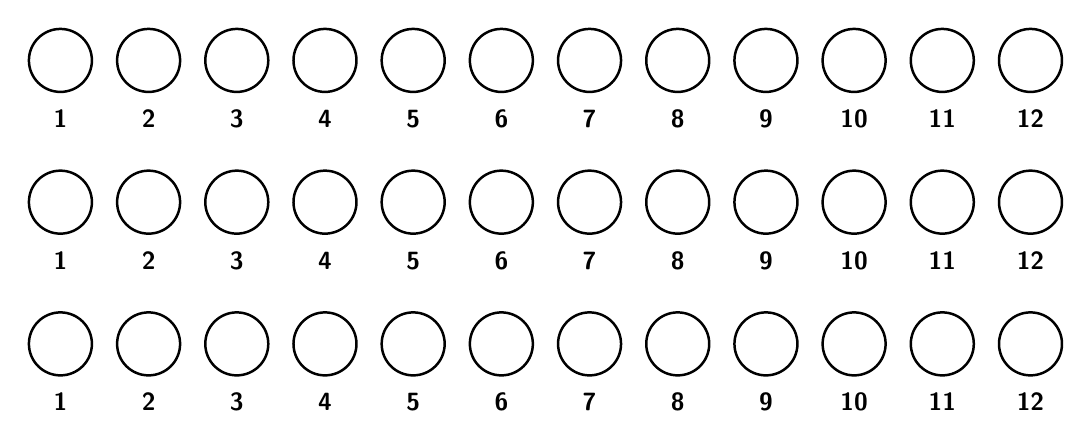
\begin{tikzpicture}
\draw[line width=0.9pt] (0.400,0.400) circle (0.400);
\node[font=\small\bfseries, anchor=base] at (0.400,-0.450) {1};
\draw[line width=0.9pt] (1.520,0.400) circle (0.400);
\node[font=\small\bfseries, anchor=base] at (1.520,-0.450) {2};
\draw[line width=0.9pt] (2.640,0.400) circle (0.400);
\node[font=\small\bfseries, anchor=base] at (2.640,-0.450) {3};
\draw[line width=0.9pt] (3.760,0.400) circle (0.400);
\node[font=\small\bfseries, anchor=base] at (3.760,-0.450) {4};
\draw[line width=0.9pt] (4.880,0.400) circle (0.400);
\node[font=\small\bfseries, anchor=base] at (4.880,-0.450) {5};
\draw[line width=0.9pt] (6.000,0.400) circle (0.400);
\node[font=\small\bfseries, anchor=base] at (6.000,-0.450) {6};
\draw[line width=0.9pt] (7.120,0.400) circle (0.400);
\node[font=\small\bfseries, anchor=base] at (7.120,-0.450) {7};
\draw[line width=0.9pt] (8.240,0.400) circle (0.400);
\node[font=\small\bfseries, anchor=base] at (8.240,-0.450) {8};
\draw[line width=0.9pt] (9.360,0.400) circle (0.400);
\node[font=\small\bfseries, anchor=base] at (9.360,-0.450) {9};
\draw[line width=0.9pt] (10.480,0.400) circle (0.400);
\node[font=\small\bfseries, anchor=base] at (10.480,-0.450) {10};
\draw[line width=0.9pt] (11.600,0.400) circle (0.400);
\node[font=\small\bfseries, anchor=base] at (11.600,-0.450) {11};
\draw[line width=0.9pt] (12.720,0.400) circle (0.400);
\node[font=\small\bfseries, anchor=base] at (12.720,-0.450) {12};
\draw[line width=0.9pt] (0.400,-1.400) circle (0.400);
\node[font=\small\bfseries, anchor=base] at (0.400,-2.250) {1};
\draw[line width=0.9pt] (1.520,-1.400) circle (0.400);
\node[font=\small\bfseries, anchor=base] at (1.520,-2.250) {2};
\draw[line width=0.9pt] (2.640,-1.400) circle (0.400);
\node[font=\small\bfseries, anchor=base] at (2.640,-2.250) {3};
\draw[line width=0.9pt] (3.760,-1.400) circle (0.400);
\node[font=\small\bfseries, anchor=base] at (3.760,-2.250) {4};
\draw[line width=0.9pt] (4.880,-1.400) circle (0.400);
\node[font=\small\bfseries, anchor=base] at (4.880,-2.250) {5};
\draw[line width=0.9pt] (6.000,-1.400) circle (0.400);
\node[font=\small\bfseries, anchor=base] at (6.000,-2.250) {6};
\draw[line width=0.9pt] (7.120,-1.400) circle (0.400);
\node[font=\small\bfseries, anchor=base] at (7.120,-2.250) {7};
\draw[line width=0.9pt] (8.240,-1.400) circle (0.400);
\node[font=\small\bfseries, anchor=base] at (8.240,-2.250) {8};
\draw[line width=0.9pt] (9.360,-1.400) circle (0.400);
\node[font=\small\bfseries, anchor=base] at (9.360,-2.250) {9};
\draw[line width=0.9pt] (10.480,-1.400) circle (0.400);
\node[font=\small\bfseries, anchor=base] at (10.480,-2.250) {10};
\draw[line width=0.9pt] (11.600,-1.400) circle (0.400);
\node[font=\small\bfseries, anchor=base] at (11.600,-2.250) {11};
\draw[line width=0.9pt] (12.720,-1.400) circle (0.400);
\node[font=\small\bfseries, anchor=base] at (12.720,-2.250) {12};
\draw[line width=0.9pt] (0.400,-3.200) circle (0.400);
\node[font=\small\bfseries, anchor=base] at (0.400,-4.050) {1};
\draw[line width=0.9pt] (1.520,-3.200) circle (0.400);
\node[font=\small\bfseries, anchor=base] at (1.520,-4.050) {2};
\draw[line width=0.9pt] (2.640,-3.200) circle (0.400);
\node[font=\small\bfseries, anchor=base] at (2.640,-4.050) {3};
\draw[line width=0.9pt] (3.760,-3.200) circle (0.400);
\node[font=\small\bfseries, anchor=base] at (3.760,-4.050) {4};
\draw[line width=0.9pt] (4.880,-3.200) circle (0.400);
\node[font=\small\bfseries, anchor=base] at (4.880,-4.050) {5};
\draw[line width=0.9pt] (6.000,-3.200) circle (0.400);
\node[font=\small\bfseries, anchor=base] at (6.000,-4.050) {6};
\draw[line width=0.9pt] (7.120,-3.200) circle (0.400);
\node[font=\small\bfseries, anchor=base] at (7.120,-4.050) {7};
\draw[line width=0.9pt] (8.240,-3.200) circle (0.400);
\node[font=\small\bfseries, anchor=base] at (8.240,-4.050) {8};
\draw[line width=0.9pt] (9.360,-3.200) circle (0.400);
\node[font=\small\bfseries, anchor=base] at (9.360,-4.050) {9};
\draw[line width=0.9pt] (10.480,-3.200) circle (0.400);
\node[font=\small\bfseries, anchor=base] at (10.480,-4.050) {10};
\draw[line width=0.9pt] (11.600,-3.200) circle (0.400);
\node[font=\small\bfseries, anchor=base] at (11.600,-4.050) {11};
\draw[line width=0.9pt] (12.720,-3.200) circle (0.400);
\node[font=\small\bfseries, anchor=base] at (12.720,-4.050) {12};
\end{tikzpicture}
\end{center}
\vspace{1.0cm}
\par\noindent\textbf{Problem 10:} Use red, blue and green with the rule of Problem 4, where 2 + 2 = 4 counts again. How far can you go?\par

\vspace{6pt}\begin{center}
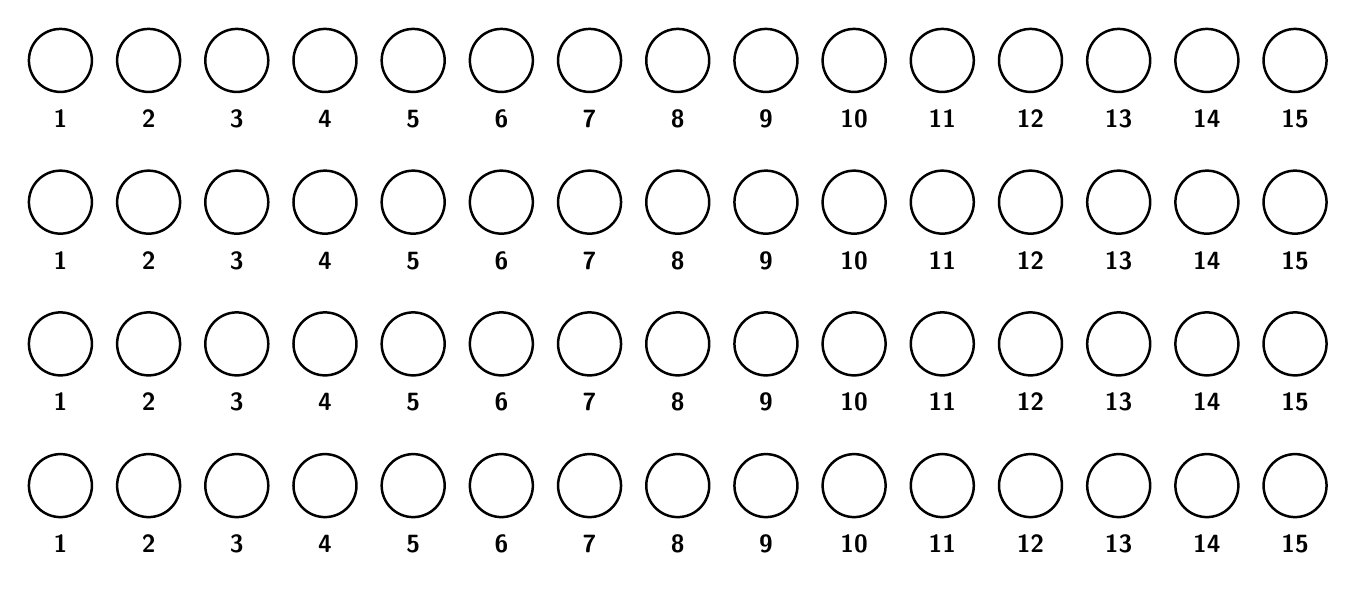
\begin{tikzpicture}
\draw[line width=0.9pt] (0.400,0.400) circle (0.400);
\node[font=\small\bfseries, anchor=base] at (0.400,-0.450) {1};
\draw[line width=0.9pt] (1.520,0.400) circle (0.400);
\node[font=\small\bfseries, anchor=base] at (1.520,-0.450) {2};
\draw[line width=0.9pt] (2.640,0.400) circle (0.400);
\node[font=\small\bfseries, anchor=base] at (2.640,-0.450) {3};
\draw[line width=0.9pt] (3.760,0.400) circle (0.400);
\node[font=\small\bfseries, anchor=base] at (3.760,-0.450) {4};
\draw[line width=0.9pt] (4.880,0.400) circle (0.400);
\node[font=\small\bfseries, anchor=base] at (4.880,-0.450) {5};
\draw[line width=0.9pt] (6.000,0.400) circle (0.400);
\node[font=\small\bfseries, anchor=base] at (6.000,-0.450) {6};
\draw[line width=0.9pt] (7.120,0.400) circle (0.400);
\node[font=\small\bfseries, anchor=base] at (7.120,-0.450) {7};
\draw[line width=0.9pt] (8.240,0.400) circle (0.400);
\node[font=\small\bfseries, anchor=base] at (8.240,-0.450) {8};
\draw[line width=0.9pt] (9.360,0.400) circle (0.400);
\node[font=\small\bfseries, anchor=base] at (9.360,-0.450) {9};
\draw[line width=0.9pt] (10.480,0.400) circle (0.400);
\node[font=\small\bfseries, anchor=base] at (10.480,-0.450) {10};
\draw[line width=0.9pt] (11.600,0.400) circle (0.400);
\node[font=\small\bfseries, anchor=base] at (11.600,-0.450) {11};
\draw[line width=0.9pt] (12.720,0.400) circle (0.400);
\node[font=\small\bfseries, anchor=base] at (12.720,-0.450) {12};
\draw[line width=0.9pt] (13.840,0.400) circle (0.400);
\node[font=\small\bfseries, anchor=base] at (13.840,-0.450) {13};
\draw[line width=0.9pt] (14.960,0.400) circle (0.400);
\node[font=\small\bfseries, anchor=base] at (14.960,-0.450) {14};
\draw[line width=0.9pt] (16.080,0.400) circle (0.400);
\node[font=\small\bfseries, anchor=base] at (16.080,-0.450) {15};
\draw[line width=0.9pt] (0.400,-1.400) circle (0.400);
\node[font=\small\bfseries, anchor=base] at (0.400,-2.250) {1};
\draw[line width=0.9pt] (1.520,-1.400) circle (0.400);
\node[font=\small\bfseries, anchor=base] at (1.520,-2.250) {2};
\draw[line width=0.9pt] (2.640,-1.400) circle (0.400);
\node[font=\small\bfseries, anchor=base] at (2.640,-2.250) {3};
\draw[line width=0.9pt] (3.760,-1.400) circle (0.400);
\node[font=\small\bfseries, anchor=base] at (3.760,-2.250) {4};
\draw[line width=0.9pt] (4.880,-1.400) circle (0.400);
\node[font=\small\bfseries, anchor=base] at (4.880,-2.250) {5};
\draw[line width=0.9pt] (6.000,-1.400) circle (0.400);
\node[font=\small\bfseries, anchor=base] at (6.000,-2.250) {6};
\draw[line width=0.9pt] (7.120,-1.400) circle (0.400);
\node[font=\small\bfseries, anchor=base] at (7.120,-2.250) {7};
\draw[line width=0.9pt] (8.240,-1.400) circle (0.400);
\node[font=\small\bfseries, anchor=base] at (8.240,-2.250) {8};
\draw[line width=0.9pt] (9.360,-1.400) circle (0.400);
\node[font=\small\bfseries, anchor=base] at (9.360,-2.250) {9};
\draw[line width=0.9pt] (10.480,-1.400) circle (0.400);
\node[font=\small\bfseries, anchor=base] at (10.480,-2.250) {10};
\draw[line width=0.9pt] (11.600,-1.400) circle (0.400);
\node[font=\small\bfseries, anchor=base] at (11.600,-2.250) {11};
\draw[line width=0.9pt] (12.720,-1.400) circle (0.400);
\node[font=\small\bfseries, anchor=base] at (12.720,-2.250) {12};
\draw[line width=0.9pt] (13.840,-1.400) circle (0.400);
\node[font=\small\bfseries, anchor=base] at (13.840,-2.250) {13};
\draw[line width=0.9pt] (14.960,-1.400) circle (0.400);
\node[font=\small\bfseries, anchor=base] at (14.960,-2.250) {14};
\draw[line width=0.9pt] (16.080,-1.400) circle (0.400);
\node[font=\small\bfseries, anchor=base] at (16.080,-2.250) {15};
\draw[line width=0.9pt] (0.400,-3.200) circle (0.400);
\node[font=\small\bfseries, anchor=base] at (0.400,-4.050) {1};
\draw[line width=0.9pt] (1.520,-3.200) circle (0.400);
\node[font=\small\bfseries, anchor=base] at (1.520,-4.050) {2};
\draw[line width=0.9pt] (2.640,-3.200) circle (0.400);
\node[font=\small\bfseries, anchor=base] at (2.640,-4.050) {3};
\draw[line width=0.9pt] (3.760,-3.200) circle (0.400);
\node[font=\small\bfseries, anchor=base] at (3.760,-4.050) {4};
\draw[line width=0.9pt] (4.880,-3.200) circle (0.400);
\node[font=\small\bfseries, anchor=base] at (4.880,-4.050) {5};
\draw[line width=0.9pt] (6.000,-3.200) circle (0.400);
\node[font=\small\bfseries, anchor=base] at (6.000,-4.050) {6};
\draw[line width=0.9pt] (7.120,-3.200) circle (0.400);
\node[font=\small\bfseries, anchor=base] at (7.120,-4.050) {7};
\draw[line width=0.9pt] (8.240,-3.200) circle (0.400);
\node[font=\small\bfseries, anchor=base] at (8.240,-4.050) {8};
\draw[line width=0.9pt] (9.360,-3.200) circle (0.400);
\node[font=\small\bfseries, anchor=base] at (9.360,-4.050) {9};
\draw[line width=0.9pt] (10.480,-3.200) circle (0.400);
\node[font=\small\bfseries, anchor=base] at (10.480,-4.050) {10};
\draw[line width=0.9pt] (11.600,-3.200) circle (0.400);
\node[font=\small\bfseries, anchor=base] at (11.600,-4.050) {11};
\draw[line width=0.9pt] (12.720,-3.200) circle (0.400);
\node[font=\small\bfseries, anchor=base] at (12.720,-4.050) {12};
\draw[line width=0.9pt] (13.840,-3.200) circle (0.400);
\node[font=\small\bfseries, anchor=base] at (13.840,-4.050) {13};
\draw[line width=0.9pt] (14.960,-3.200) circle (0.400);
\node[font=\small\bfseries, anchor=base] at (14.960,-4.050) {14};
\draw[line width=0.9pt] (16.080,-3.200) circle (0.400);
\node[font=\small\bfseries, anchor=base] at (16.080,-4.050) {15};
\draw[line width=0.9pt] (0.400,-5.000) circle (0.400);
\node[font=\small\bfseries, anchor=base] at (0.400,-5.850) {1};
\draw[line width=0.9pt] (1.520,-5.000) circle (0.400);
\node[font=\small\bfseries, anchor=base] at (1.520,-5.850) {2};
\draw[line width=0.9pt] (2.640,-5.000) circle (0.400);
\node[font=\small\bfseries, anchor=base] at (2.640,-5.850) {3};
\draw[line width=0.9pt] (3.760,-5.000) circle (0.400);
\node[font=\small\bfseries, anchor=base] at (3.760,-5.850) {4};
\draw[line width=0.9pt] (4.880,-5.000) circle (0.400);
\node[font=\small\bfseries, anchor=base] at (4.880,-5.850) {5};
\draw[line width=0.9pt] (6.000,-5.000) circle (0.400);
\node[font=\small\bfseries, anchor=base] at (6.000,-5.850) {6};
\draw[line width=0.9pt] (7.120,-5.000) circle (0.400);
\node[font=\small\bfseries, anchor=base] at (7.120,-5.850) {7};
\draw[line width=0.9pt] (8.240,-5.000) circle (0.400);
\node[font=\small\bfseries, anchor=base] at (8.240,-5.850) {8};
\draw[line width=0.9pt] (9.360,-5.000) circle (0.400);
\node[font=\small\bfseries, anchor=base] at (9.360,-5.850) {9};
\draw[line width=0.9pt] (10.480,-5.000) circle (0.400);
\node[font=\small\bfseries, anchor=base] at (10.480,-5.850) {10};
\draw[line width=0.9pt] (11.600,-5.000) circle (0.400);
\node[font=\small\bfseries, anchor=base] at (11.600,-5.850) {11};
\draw[line width=0.9pt] (12.720,-5.000) circle (0.400);
\node[font=\small\bfseries, anchor=base] at (12.720,-5.850) {12};
\draw[line width=0.9pt] (13.840,-5.000) circle (0.400);
\node[font=\small\bfseries, anchor=base] at (13.840,-5.850) {13};
\draw[line width=0.9pt] (14.960,-5.000) circle (0.400);
\node[font=\small\bfseries, anchor=base] at (14.960,-5.850) {14};
\draw[line width=0.9pt] (16.080,-5.000) circle (0.400);
\node[font=\small\bfseries, anchor=base] at (16.080,-5.850) {15};
\end{tikzpicture}
\end{center}
\end{document}
